% XeLaTeX document
\documentclass[10pt,ebook,openany]{memoir}

% Редактируем: конфигурация, личные настройки: имя, название предмета и пр. для титульной страницы и метаданных документа здесь
\newcommand{\university}{Санкт-Петербургский политехнический университет Петра Великого}
\newcommand{\faculty}{Институт прикладной математики и механики}
\newcommand{\department}{Высшая школа прикладной математики и вычислительной физики}
\newcommand{\city}{Санкт-Петербург}
\newcommand{\docname}{Теория вероятностей. Kонспект.}
\newcommand{\type}{Теория вероятностей. Kонспект.}
\newcommand{\num}{ № 1}
\newcommand{\subject}{Теория вероятностей. Конспект.}
\newcommand{\tutorname}{к.б.н. Н. О. Кадырова}
\newcommand{\studentname}{В. Тюльпин,  Ю. Камалетдинова}

% Не редактируем: используемые пакеты
% настройка кодировки, шрифтов и русского языка
\usepackage{fontspec}
\usepackage{polyglossia}

% рабочие ссылки в документе
\usepackage{hyperref}

% графика
\usepackage{graphicx}
\usepackage{tikz}

% поворот страницы
\usepackage{pdflscape}

% качественные листинги кода
\usepackage{minted}
\usepackage{listings}
\usepackage{lstfiracode}

% отключение копирования номеров строк из листинга, работает не во всех просмотрщиках (в Adobe Reader работает)
\usepackage{accsupp}
\newcommand\emptyaccsupp[1]{\BeginAccSupp{ActualText={}}#1\EndAccSupp{}}
\let\theHFancyVerbLine\theFancyVerbLine
\def\theFancyVerbLine{\rmfamily\tiny\emptyaccsupp{\arabic{FancyVerbLine}}}

% библиография
%\bibliographystyle{templates/gost-numeric.bbx}
%\usepackage{csquotes}
%\usepackage[parentracker=true,backend=biber,hyperref=false,bibencoding=utf8,style=numeric-comp,language=english,autolang=other,citestyle=gost-numeric,defernumbers=true,bibstyle=gost-numeric,sorting=ntvy,]{biblatex}

% установка полей
\usepackage{geometry}

% нумерация картинок по секциям
\usepackage{chngcntr} 

% дополнительные команды для таблиц
\usepackage{booktabs}

% для перечислений с именованными пунктами
\usepackage{enumitem}

% для заголовков
\usepackage{caption} 
\usepackage{titlesec}
\usepackage[dotinlabels]{titletoc}

% разное для математики
\usepackage{amsmath, amsfonts, amssymb, amsthm, mathtools}
\usepackage[makeroom]{cancel}

% водяной знак на документе, см. main.tex
\usepackage[printwatermark]{xwatermark} 

% Не редактируем: параметры используемых пакетов и не только
% настройки polyglossia
\setdefaultlanguage{russian}
\setotherlanguage{english}

% локализация
\addto\captionsrussian{
  \renewcommand{\figurename}{Рисунок}%
  \renewcommand{\partname}{Глава}
  \renewcommand{\contentsname}{\centerline{Содержание}}
  \renewcommand{\listingscaption}{Листинг}
}

% основной шрифт документа
\setmainfont{CMU Serif}

% перечень использованных источников
% \addbibresource{refs.bib}

% настройка полей
\geometry{top=2cm}
\geometry{bottom=2cm}
\geometry{left=2cm}
\geometry{right=2cm}
\geometry{bindingoffset=0cm}

% настройка ссылок и метаданных документа
\hypersetup{unicode=true,colorlinks=true,linkcolor=red,citecolor=green,filecolor=magenta,urlcolor=cyan,        		       
    pdftitle={\docname},   	    
    pdfauthor={\studentname},      
    pdfsubject={\subject},      		        
    pdfcreator={\studentname}, 	       
    pdfproducer={Overleaf}, 		     
    pdfkeywords={\subject}
}

% настройка подсветки кода и окружения для листингов
\usemintedstyle{colorful}
\newenvironment{code}{\captionsetup{type=listing}}{}

% шрифт для листингов с лигатурами
\setmonofont{FiraCode-Regular.otf}[
    Path = templates/,
    Contextuals=Alternate
]

% оформления подписи рисунка
\captionsetup[figure]{labelsep = period}

% подпись таблицы
\DeclareCaptionFormat{hfillstart}{\hfill#1#2#3\par}
\captionsetup[table]{format=hfillstart,labelsep=newline,justification=centering,skip=-10pt,textfont=bf}

% путь к каталогу с рисунками
\graphicspath{{fig/}}

\titlelabel{\thetitle.\quad}

% для удобного конспектирования математики
\mathtoolsset{showonlyrefs=true}

\theoremstyle{definition}
\newtheorem*{theorem}{Теорема}
\theoremstyle{definition}
\newtheorem*{lemma}{Лемма}
\theoremstyle{definition}
\newtheorem*{definition}{Определение}
\theoremstyle{definition}
\newtheorem*{conclusion}{Следствие}
\theoremstyle{definition}
\newtheorem*{example}{Пример}
\theoremstyle{definition}
\newtheorem*{addition}{Замечание}
\theoremstyle{definition}
\newtheorem*{interjection}{Отступление}

% настоящее матожидание
\newcommand{\MExpect}{\mathsf{M}}

% объявили оператор!
\DeclareMathOperator{\sgn}{\mathop{sgn}}

% перенос знаков в формулах (по Львовскому)
\newcommand*{\hm}[1]{#1\nobreak\discretionary{} {\hbox{$\mathsurround=0pt #1$}}{}} 

\renewcommand{\thesection}{\arabic{section}}

\titleformat{\section}{\normalfont\Large\bfseries}{\S\thesection}{1em}{}
\setlength{\parindent}{0pt}

\setcounter{tocdepth}{1} 

\makeatletter
\@addtoreset{section}{part}
\makeatother
\pagestyle{plain}
\flushbottom

% 
\newcommand\To[1]{1,2,\dots,#1}
\newcommand\ZTo[1]{0,1,\dots,#1}

\newcommand*{\textitplusparen}[1]{\textit{#1)}}

% водяной знак для обозначения статуса документа
% \newwatermark[allpages,color=red!5,angle=45,scale=3,xpos=0,ypos=0]{DRAFT}
\begin{document}
% Не редактируем: Титульная страница (формируется автоматически из заданной конфигурации)
\newpage
\pagenumbering{gobble}
{
  	\center
		\university
		\\ \faculty
		\\ \textbf{\department}

	\vfill ~
	\textbf{
		\\ \large \subject
		\\ \normalsize
	}
	{		
		лектор: \tutorname
	}
	\vfill ~

\medskip
\studentname \\	\city
\\ \the\year \ г. \\
%\end{titlepage}
}
\newpage
\pagenumbering{arabic}


% Не редактируем: Страница содержания (формируется автоматически из section, subsection и пр., указанных в content.tex)
\tableofcontents


% Редактируем: всё остальное: вступление, др. этапы, заключение, приложение
\newpage
\chapter{Исчисление вероятностей случайных событий}
\section{Соотношение между случайными событиями}


Пусть имеется фиксированный комплекс условий, воспроизводимый любое количество раз, в том числе и неограниченное.

\begin{definition}
	Комплекс испытаний будем называть \textit{экспериментом}.
\end{definition}

\begin{definition}
	Явления в результате испытаний обозначим как \textit{события}.
\end{definition}

Рассмотрим связанную с этим комплексом условий \textit{систему событий}.
\[
	\{A, B, C, \dots\},
	\{A_1, A_2, \dots, A_n\}
\]

\subsection{Соотношения между событиями}

\begin{enumerate}
	\item $U$ --- \textit{достоверное событие}, в результате испытаний происходит всегда.
	\item $V$ --- \textit{невозможное событие}, никогда не происходит.
	\item \textit{Сумма событий} ($\sum\limits_{i=1}^n A_i$) --- событие, происходящее тогда и только тогда, когда происходит хотя бы одно из связанных событий.
	\item \textit{Произведение событий} ($\prod\limits_{i=1}^n A_i$) --- событие, происходящее тогда и только тогда, когда происходят все из связанных событий.
	\item Событие $A$ --- \textit{частный случай} события $B$, если с появлением $A$ появляется и $B$ ($A \subset B$). Если $A$ влечёт $B$ и $B$ влечёт $A$, то события $A$ и $B$ равносильны ($A = B$).
\end{enumerate}
\begin{proof}
	$A \subset B \Rightarrow A\cdot B = A, A + B = B.$
	$B = A \Rightarrow B + A = A, A + A = A.$
\end{proof}
\begin{enumerate}
	\setcounter{enumi}{5}
	\item $\bar{A}$ --- \textit{противоположное событие}, если оно происходит только тогда, когда $A$ не происходит.

	      \[
		      A  ,  \bar{A} \text{ противоположны} \Leftrightarrow
		      \begin{cases}
			      A\cdot \bar{A} = V \\
			      A + \bar{A} = U
		      \end{cases}
	      \]

	\item События $A$ и $B$ называются \textit{несовместными}, если их одновременное появление невозможно.
	      $$A\cdot B = V$$

	\item \textit{Разность событий} $A$ и $B$ состоит в том, что $A$ происходит, а $B$ нет. ($A - B$).
\end{enumerate}

\subsection{Свойства событий}
\textbf{Коммутативность.} $A + B = B + A, \; A\cdot B = B\cdot A$ \\

\textbf{Ассоциативность.} $A + (B + C)=(A + B) + C, \; A\cdot (B\cdot C) = (A\cdot B)\cdot C$ \\

\textbf{Дистрибутивность.} $(A + B)\cdot C = A\cdot C + B\cdot C, \;  A + B\cdot C = (A + B)\cdot (A + C)$

\subsection{Некоторые тождества}
\begin{enumerate}
	\item $A + A\cdot B = A$
\end{enumerate}
\begin{proof}
	\textit{Самостоятельно.}
\end{proof}

\begin{enumerate}
	\setcounter{enumi}{1}
	\item{$A + B = A + \bar{A}\cdot B$}
\end{enumerate}
\begin{proof}
	\textit{Самостоятельно.}
\end{proof}

\begin{enumerate}
	\setcounter{enumi}{2}
	\item Формула инверсий (законы Де Моргана).
	      \smallskip

	      $\overline{(A\cdot B)} = \overline{A} + \overline{B}$, можно обобщить до $\overline{\prod\limits_{i=1}^n A_i} = \sum\limits_{i=1}^n \overline{A_i} $

	      $\overline{(A + B)} = \overline{A}\cdot \overline{B}$, можно обобщить до $\overline{\sum\limits_{i=1}^n A_i} = \prod\limits_{i=1}^n \overline{A_i} $
\end{enumerate}
События $A_1 \dots A_n$ образуют \textit{полную группу событий}, если при каждом испытании произойдёт хотя бы одно из них.
\smallskip

\example $A, \overline{A}$ --- полная группа.
\example Событие $A_k$ --- событие $A$ произошло $k$ раз в серии из $n$ испытиание. Тогда $A_0, \ldots, A_n$--- полная группа.

\section{Классическое определение вероятности}
Пусть результат испытания --- одно из попарно несовместных образующих полную группу равновозможных событий. Такая группа называется элементарной, а её результат --- элементарным исходом. \\
$E_1, \dots, E_n$ --- элементарные события $\Leftrightarrow$ $E_k\cdot E_i = V,$ где $i, k = \ZTo n$, $i \not= k$, при этом $\sum\limits_{i = 1}^n E_i = U$

\definition $E_n$ называется благоприятствующим для некоторого события $A$, если $E_n$ влечёт $A$.
\definition Вероятностью появления события $A$ будем называть отношение числа элементарных благоприятных событий $m$ к числу исходов $n$.
\begin{equation}
	\Prob (A) = \frac{m}{n} \hfill
\end{equation}
\addition При расчёте вероятности события $A$ по формуле (1) выбор системы элементарных событий можно произвести различными способами.
\conclusion $\Prob(U) = 1, \; \Prob(V) = 0.$
\conclusion $\forall A \quad 0 \leqslant \Prob(A) \leqslant 1.$
\section{Вероятность и относительная частота}
\begin{definition}
	Пусть при одних и тех же условиях произведено $N$ испытаний, в результате которых интересующее событие произошло $M$ раз.
\end{definition}

Относительной частотой появления события $A$ назовём число

\begin{equation}
	\tilde{\Prob}(A) = \frac{M}{N}
\end{equation}

Относительная частота является величиной, рассчитываемой по факту произошедшего эксперимента, и, вообще говоря, не является оценкой вероятности, однако при достаточно большом количестве испытаний относительную частоту можно считать приближённо равной вероятности этого события.
Очевидно, что
$$\tilde{\Prob}(V) = \Prob(V) = 0,$$
$$\tilde{\Prob}(U) = \Prob(U) = 1.$$
Но из равенства $\tilde{\Prob}(A) = 0$ не следует, что $\Prob(A) = 0$, как и в случае с  $\tilde{\Prob}(A) = 1$.
\[
	\Prob(A) = \xcancel {\lim_{n\to\infty} \tilde{\Prob}(A)} = \lim_{N\to\infty} \frac{M}{N}.
\]
При увеличении числа опытов отклонения (большие) относительной частоты $\tilde{\Prob}(A)$ от вероятности $\Prob(A)$ будут попадаться реже. На практике относительная частота $\tilde{\Prob}(A)$ может быть принята за вероятность $\Prob(A)$ при достаточно большом количестве испытаний.

\section{Геометрические вероятности}
Пусть $\chi_0$ --- номинальный размер некоторой детали. С учётом погрешности изготовления этой детали реальный размер $\chi \in (\chi - 4; \chi + 4)$. Получено несчётное пространство, и классическое определение вероятности, заданное для счётных пространств событий, не может быть использовано для вычислений в данном случае.

\subsection{Геометрический подход}
Пусть имеется ограниченное евклидово множество, имеющее объём. \\
Рассмотрим $S$ --- систему подмножеств исходного множества $\Omega$, имеющих объём. Положим
\[
	\forall A \in S \quad \Prob(A) = \frac{\vert {A} \vert}{\vert \Omega \vert}
\]
Тройка объектов $ \big<\Omega, S, \Prob\big> $ служит моделью задач, в которых точку бросают в область $\Omega$.
\smallskip

При этом вероятность того, что некоторая точка попала в область $A$, пропорциональна объёму $A$.
\subsection{Парадоксы}
\begin{itemize}
	\item Геометрическая вероятность попадания в какую-либо точку отрезка равна нулю.
	      То есть, вероятность невозможного события равна нулю, однако обратное не является верным.
	\item Взаимно однозначное преобразование может существенно изменить вероятность.
\end{itemize}
\subsubsection{Парадокс Бертрана}
Для некоторой окружности случайно выберем хорду. Найдём вероятность того, что хорда длиннее стороны правильного треугольника, вписанного в эту окружность. $A$ --- интересующее нас событие.
\begin{description}[leftmargin=0cm]
	\item[Метод «случайного центра».] Выберем наудачу произвольную точку внутри круга и построим хорду с центром в выбранной точке. Хорда длиннее стороны равностороннего треугольника, если выбранная точка находится внутри круга, вписанного в треугольник. Площадь вписанного круга есть 1/4 от площади большего, значит, исходная вероятность равна 1/4.
	      \begin{figure}[ht]
		      \centering
		      \def\svgwidth{8em}
		      \input{fig/Bertrand/1-4.pdf_tex}
		      \caption{Случайные хорды, выбранные в случае 1.}
	      \end{figure}
	      \[
		      \Prob(A) = \frac{\pi \frac{R^2}{4}}{\pi R^2} = \frac{1}{4}.
	      \]
	\item[Метод «случайных концов».] Наудачу выберем две точки на окружности и проведём через них хорду. Чтобы посчитать искомую вероятность, представим, что треугольник повёрнут так, что одна из его вершин совпадает с концом хорды. Заметим, что если другой конец хорды лежит на дуге между двумя другими вершинами треугольника, то длина хорды больше стороны треугольника. Длина рассмотренной дуги равна трети длины окружности, следуя классическому определению, искомая вероятность равна 1/3.
	      \begin{figure}[ht]
		      \centering
		      \def\svgwidth{8em}
		      \input{fig/Bertrand/1-3.pdf_tex}
		      \caption{Случайные хорды, выбранные в случае 2.}
	      \end{figure}
	      \[
		      \Prob(A) = \frac{2\pi \frac{R}{3}}{2 \pi R} = \frac{1}{3}.
	      \]
	\item[Метод «случайного радиуса».] Зафиксируем радиус окружности, наудачу выберем точку на радиусе. Построим хорду, перпендикулярную зафиксированному радиусу, проходящую через выбранную точку. Для нахождения искомой вероятности представим, что треугольник повёрнут так, что одна из его сторон перпендикулярна зафиксированному радиусу. Хорда длиннее стороны треугольника, если её центр ближе к центру, чем точка пересечения треугольника с зафиксированным радиусом. Сторона треугольника делит пополам радиус, следовательно вероятность выбрать хорду длиннее стороны треугольника --- 1/2.
	      \begin{figure}[ht]
		      \centering
		      \def\svgwidth{8em}
		      \input{fig/Bertrand/1-2.pdf_tex}
		      \caption{Случайные хорды, выбранные в случае 3.}
	      \end{figure}
	      \[ \Prob(A) = \frac{\frac{R}{2}}{R} = \frac{1}{2}. \]
\end{description}
Возможны различные выборы равномерным образом, и каждый метод использует свой выбор.
\section{Условная вероятность. Теорема умножения вероятностей. Независимость событий}
Пусть $A, B$ --- события, при этом $B \not= V$.
\begin{definition}
	Вероятность $A$, вычисляемая при условии, что $B$ произошло, называется условной вероятностью $A$ относительно $B$.
\end{definition}
\[ \Prob(A  \mid  B) \]
Если $\Prob(A \mid B) = \Prob(A)$, то $A$ не зависит от $B$. В противном случае $A$ зависит от $B$.
\subsection{Теорема умножения вероятностей}
Рассмотрим систему $n$ элементарных событий $\{E_i\}_{i = \To n}$. Событию $A$ благоприятствуют $m$ элементарных событий, событию $B$ --- $k$ событий, $A\cdot B$ --- $l$ событий ($m, k, l \leqslant n$). Тогда
\[ \Prob(A) = \frac{m}{n},\;\Prob(B) = \frac{k}{n},\;\Prob(A\cdot B) = \frac{l}{n}. \]
\[ \Prob(B \mid A) = \frac{l}{m} = \frac{\frac{l}{n}}{\frac{m}{n}} = \frac{\Prob(A \times B)}{\Prob(A)},\]
\[ \Prob(A \mid B) = \frac{\frac{l}{n}}{\frac{k}{n}}, \text{ то есть} \]
\[ \Prob(A \times B) = \Prob(A) \cdot \Prob(B \mid A) = \Prob(B) \cdot \Prob(A \mid B) \]
Установлена теорема умножения двух любых событий, хотя бы одно из которых является возможным. \\
Пусть $A$ не зависит от $B$. Тогда
\[
	\Prob(A) \cdot \Prob(B \mid A) \overset{\makebox[0pt]{\mbox{*}}}{=} \Prob(B) \cdot \Prob(A) \Rightarrow \text{$B$ не зависит от $A$}
\]
\subsection{Независимость событий}
\begin{definition}
	Два события $A$ и $B$ независимы $\Leftrightarrow \Prob(A \cdot B) = \Prob(A) \cdot \Prob(B)$ (также верно, если одно из событий является невозможным).
\end{definition}
\begin{example}
	Пусть имеется колода из 36 карт, из неё случайным образом вытаскиваем одну карту. Пусть событие $A$ -- <<вытянут \texttt{A} (туз)>>, событие $B$ -- <<вытянута карта масти {\color{red} $\blacklozenge$}>>. Тогда событие $A \cdot B$ -- вытянута карта ${\color{red} \blacklozenge} \texttt{A}$.
	\[
		\Prob(A) = \frac{4}{36} = \frac{1}{9}, \Prob(B) = \frac{9}{36} = \frac{1}{4},
	\]
	\[
		\Prob(A \cdot B) = \frac{1}{36}
	\]
\end{example}
Приведём теорему об умножении $n$ любых событий, хотя бы одно из которых возможно
\[
	\Prob(A_1 \cdot \ldots \cdot A_n) = \Prob(A_1) \cdot \Prob(A_2 \mid A_1) \cdot \Prob(A_3 \mid A_1 \cdot A_2) \cdot \dots
\]
\[
	\ldots \cdot \Prob(A_n \mid \prod\limits_{k = 1}^{n-1} A_k)
\]
\begin{proof}
\textit{Самостоятельно.}
\end{proof}
\[ \begin{split}
	\Prob(A_1 \cdot A_2 \cdot A_3) &= \Prob(A_1 \cdot A_2) \cdot \Prob(A_3 \mid A_1 \cdot A_2) = \\
	&= \Prob(A_1) \cdot \Prob(A_2 \mid A_1) \cdot \Prob(A_3 \mid A_1 \cdot A_2)
\end{split} \]
Попарная независимость событий
\begin{equation}\label{1-5-3}
	\left\{ \begin{aligned}
		&\Prob(A_1 \cdot A_2) = \Prob(A_1) \cdot \Prob(A_2) \\
		&\Prob(A_1 \cdot A_3) = \Prob(A_1) \cdot \Prob(A_3) \\
		&\Prob(A_2 \cdot A_3) = \Prob(A_2) \cdot \Prob(A_3)
	\end{aligned} \right.
\end{equation}

При независимости событий (в совокупности):
\begin{equation}\label{1-5-4}
	\Prob(A_1 \cdot A_2 \cdot A_3) = \Prob(A_1) \cdot \Prob(A_2) \cdot \Prob(A_3)
\end{equation}
\subsection{Парадокс Бернштейна}
Рассмотрим испытание, в результате которого бросаются две монеты. Пусть
\begin{itemize}
	\item событие $A$ -- <<на первой монете выпал орёл>>,
	\item событие $B$ -- <<на второй монете выпал орёл>>,
	\item событие $C$ -- <<только на одной монете выпал орёл>>.
\end{itemize}
Установим систему элементарных событий $\Omega$, равную \{О--О, Р--Р, Р--О, О--Р\}.
\[
	\Prob(A) = \Prob(B) = \Prob(C) = \frac{1}{2}
\]
\[ \Prob(A \cdot B) = \frac{1}{4} = \Prob(A) \cdot \Prob(B), \]
\[ \Prob(A \cdot C) = \frac{1}{4} = \Prob(A) \cdot \Prob(C), \]
\[ \Prob(B \cdot C) = \frac{1}{4} = \Prob(B) \cdot \Prob(C). \]

\[ \Prob(A \cdot B \cdot C) = 0 \not= \Prob(A) \cdot \Prob(B) \cdot \Prob(C)\]
\textbf{Вывод:} попарная независимость (\ref{1-5-3}) $\cancel{\Rightarrow}$ независимость в совокупности (\ref{1-5-4}). \\
События независимы в совокупности $\Leftrightarrow$ (\ref{1-5-3}) и (\ref{1-5-4}) выполняются.
\begin{definition}
	$A_1, \dots, A_n$ независимы в совокупности, если
	\[
		\Prob(A_{i_1} \cdot \dots A_{i_k}) = \Prob(A_{i_1}) \cdot \ldots \cdot \Prob(A_{i_n}), \text{ где}
	\]
	\[
		1 \leqslant i_1 < i_2 < \ldots < i_k \leqslant n
	\]
\end{definition}
$\boxed{2^n - C_n^1 - C_n^0}$ -- число соотношений для проверки независимости событий в совокупности. Если нам заранее известно, что $A_1, \dots, A_n$ независимы в совокупности, то
\[
	\Prob(\prod\limits_{k = 1}^n A_k) = \prod\limits_{k = 1}^n \Prob(A_k)
\]
\section{Теорема сложения вероятностей}
Рассмотрим события $A$ и $B$.
\begin{itemize}
	\item $A$ -- $m$ элементарных событий из $n$,
	\item $B$ -- $k$ элементарных событий из $n$,
	\item $A \cdot B$ -- $l$ элементарных событий из $n$.
\end{itemize}
\[
	\Prob(A + B) = \frac{m + k - l}{n} = \Prob(A) + \Prob(B) - \Prob(A \cdot B)
\]
Установлена теорема о сложении двух любых событий.

Для несовместных событий:
\[
	A \cdot B = V \Rightarrow \Prob(A + B) = \Prob(A) + \Prob(B)
\]
Если $B$ = $\overline{A}$, то
\[
	\underbrace{\Prob(A + \overline{A})}_{\Prob(U) = 1} = \Prob(A) + \Prob(\overline{A}) \Rightarrow \Prob(\overline{A}) = 1 - \Prob(A)
\]
По теореме о сложении:
\[ \Prob(A_1 + A_2 + A_3) = \Prob(A_1 + A_2) + \Prob(A_3) -  \]
\[ - \Prob((A_1 + A_2) \cdot A_3) = \Prob(A_1) + \Prob(A_2) + \Prob(A_3) - \]	
\[ - \Prob(A_1 \cdot A_2) - \Prob(A_1 \cdot A_3) - \Prob(A_2 \cdot A_3) + \]
\[ + \Prob(A_1 \cdot A_2 \cdot A_3) \]
Обобщённая формула:
\[ \Prob(\sum\limits_{k=1}^n A_k) = \sum\limits_{k=1}^n \Prob(A_k) - \sum\limits_{k=1}^{n-1} \sum\limits_{j=k+1}^n \Prob(A_k \cdot A_j) + \]
\[
	+ \sum\limits_{k=1}^{n-2} \sum\limits_{j=k+1}^{n-1} \sum\limits_{i=j+1}^n \Prob(A_k \cdot A_j \cdot A_i) - \ldots 
\]
\[
	\ldots + (-1)^{n-1} \cdot \Prob(\prod\limits_{k=1}^n A_k)
\]
Для попарно несовместных событий:
\[
	\underset{i \not= j}{A_i \cdot A_j} = V \Rightarrow \Prob(\sum\limits_{k=1}^n A_k) = \sum\limits_{k=1}^n \Prob(A_k)
\]
Если $A_1, \dots, A_n$ независимы в совокупности, то справедлива следующая формула:
\[
	\Prob(\sum\limits_{k=1}^n A_k) = 1 - \Prob(\overline{\sum\limits_{k=1}^n A_k}) = 1 - \Prob(\prod\limits_{k=1}^n \overline{A_k}) =
\]
\[ = 1 - \prod\limits_{k=1}^n \Prob(\overline{A_k}) = 1 - \prod\limits_{k=1}^n(1 - \Prob(A_k)). \]
Если вероятности исходных событий не зависят от номеров и определяются только числом сомножителей, то
\[ \begin{split}
	\Prob(\sum\limits_{k=1}^n A_k) &= C_n^1 \Prob(A_1) - C_n^2 \Prob(A_1 \cdot A_2) + \\
	&+ C_n^3 \Prob(A_1 \cdot A_2 \cdot \cdot A_3) - \ldots + (-1)^{n-1} C_n^n \Prob(\prod\limits_{k=1}^n A_k)
\end{split} \]
\begin{proof}
	\textit{Самостоятельно.}
\end{proof}
\[ \Prob(\prod\limits_{k=1}^n A_k) = \sum\limits_{k=1}^n \Prob(A_k) - \sum\limits_{k=1}^{n-1} \sum\limits_{j=k+1}^{n} \Prob(A_k + A_j) + \]
\[ + \sum\limits_{k=1}^{n-2} \sum\limits_{j=k+1}^{n-1} \sum\limits_{i=j+1}^{n} \Prob(A_k + A_j + A_i) - \ldots + (-1)^{n-1} \Prob(\sum\limits_{k=1}^n A_k) \]
\begin{proof}
	\textit{Самостоятельно.}
\end{proof}
\section{Формула полной вероятности и формула Байеса}
\subsection{Формула полной вероятности}
Пусть имеется $n$ попарно несовместных событий, составляющих полную группу, $H_1, \dots, H_n$ --- назовём их гипотезами.
\begin{itemize}
	\item $\sum\limits_{i=1}^n H_i = U$,
	\item $H_i \cdot H_j = V,$ где $i, j = \To n,$ при этом $i \not= j$.
\end{itemize}
В силу попарной несовместности 
\[
	\Prob(\sum\limits_{i=1}^n H_i) = \sum\limits_{i=1}^n \Prob(H_i) = 1
\]
Рассмотрим событие $A$:
\[ A = U \cdot A = \left( \sum\limits_{i=1}^n H_i \right) \cdot A = \sum\limits_{i=1}^n H_i \cdot A \]
\[
	\Prob(A) = \Prob(\sum\limits_{i=1}^n H_i \cdot A) = \sum\limits_{i=1}^n \underbrace{\Prob(H_i \cdot A)}_{\underset{\text{зав. от опыта}}{\textit{a posteriori}}} = \underbrace{\sum\limits_{i=1}^n \Prob(H_i) \cdot \Prob(A \mid H_i)}_{\underset{\text{не зав. от опыта}}{\textit{a priori}}}
\]
\captionof*{figure}{\textbf{Формула полной вероятности.}}
\[\boxed{\Prob(A) = \sum\limits_{i=1}^n \Prob(H_i) \cdot \Prob(A \mid H_i)} \]
\subsection{Формула Байеса}
Получим формулу Байеса:
\[ \Prob(A \cdot H_k) = \Prob(A) \cdot \Prob(H_k \mid A) = \Prob(H_k) \cdot \Prob(A \mid H_k) \]

\[ \Prob(H_k \mid A) = \frac{\Prob(H_k) \cdot \Prob(A \mid H_k)}{\Prob(A)} = \frac{\Prob(H_k) \cdot \Prob(A \mid H_k)}{\sum\limits_{i=1}^n \Prob(H_i) \cdot \Prob(A \mid H_i)}
\]
\captionof*{figure}{\textbf{Формула Байеса.}}
\[ \boxed{\Prob(H_k \mid A) = \frac{\Prob(H_k) \cdot \Prob(A \mid H_k)}{\sum\limits_{i=1}^n \Prob(H_i) \cdot \Prob(A \mid H_i)}} \]

\section{Последовательность испытаний Бернулли. Биномиальный закон распределения вероятностей. Закон распределения вероятностей Пуассона}
\subsection{Последовательность испытаний Бернулли}
Пусть производится серия из $n$ испытаний, имеется $k$ исходов. Исходы образуют полную группу событий и являются попарно независимыми событиями. В рамках данного параграфа $k = 2$.
\begin{definition}
	Испытания независимы, если все исходы этих испытаний независимы в совокупности.
\end{definition}
\begin{definition}
	$n$ испытаний образуют последовательность испытаний Бернулли, если
	\begin{enumerate}
		\item Они независимы
		\item У каждого из этих испытаний 2 исхода: $\{\underset{\text{успех}}{A}, \underset{\text{неудача}}{\overline{A}} \}$
		\item Вероятность появления исхода во всех испытаниях не изменяется.
	\end{enumerate}
\end{definition}
$A_i$ -- появление $A$ в $i$-ом испытании. Тогда
\[ \forall i=\To n \quad \Prob(A_i) = p \Rightarrow \Prob(\overline{A_i}) = 1 - p = q \]
Пусть имеется $n$ испытаний с $k=2$ исходами. $B_m$ --- событие $A$ произошло $m$ раз, $0 \leqslant m \leqslant n$.
\[B_m = \overbrace{A_1 \cdot A_2 \cdot \ldots \cdot A_{m-1} \cdot A_m}^{m} \cdot \overline{A_{m+1}} \cdot \ldots \]
\[ \ldots \cdot \overline{A_n} + \ldots + \underbrace{\overline{A_1} \cdot \overline{A_2} \cdot \dots \cdot \overline{A_{n-m}}}_{n-m} \cdot \overbrace{A_{n-m+1} \cdot \ldots \cdot A_n}^m.\]
Число слагаемых --- $C_n^m$.

Будем обозначать $\Prob_m^{(n)} = \Prob(B_m)$.
\captionof*{figure}{\textbf{Формула Бернулли}}
\[
	\boxed{\Prob_m^{(n)} = C_n^m p^m q^{n-m}}
\]
\[
	\sum\limits_{m=0}^n \Prob_m^{(n)} = (p + q)^n = 1
\]
Рассмотрим вероятность того, что в $n$ испытаниях Бернулли событие $A$ произойдёт не менее $m$ раз.
\[
	R_m^{n} = \sum\limits_{k = m}^n \Prob_k^{(n)} = 1 - \sum\limits_{k=0}^{m-1} P_k^{(n)}
\]
\begin{example}
	Вероятность того, что при $n$ испытаний $A$ произойдёт хотя бы 1 раз:
	\[ R_1^{(n)} = 1 - \Prob_0^{(n)} = 1 - q^n \]
\end{example}
\subsection{Закон распределения вероятностей Пуассона}
Рассмотрим последовательность испытаний Бернулли, когда число испытаний $n \to \infty$, при этом $p = \Prob(A_i) \to 0$, $np = a$ --- константа
\[
	\Prob_m \equiv \lim_{n \to \infty} C_n^m p^m (1-p)^{n-m}
\]
\[ p = \frac{a}{n} \]
\[ \Prob_m = \lim_{n \to \infty} \frac{n!\ a^m (1 - \frac{a}{n})^n}{(n-m)!\ m!\ n^m (1 - \frac{a}{n})^m} = \frac{a^m}{m!} \cdot e^{-a}, m = 0, 1, 2, \dots \]
\captionof*{figure}{$\underset{(\textit{редких событий})}{\textbf{Закон распределения вероятностей Пуассона}}$}
\[ \boxed{\sum\limits_{m=0}^\infty \Prob_m = \sum\limits_{m=0}^\infty \frac{a^m}{m!} \cdot e^{-a} = 1}\]
\begin{example}
	Пусть $n$ --- число атомов в веществе, время распада --- 1 секунда. Тогда $p \approx 10^{-12}$.
\end{example}

\section{Полиномиальное распределение вероятностей}
Пусть имеется $n$ испытаний с $k \geqslant 2$ исходами. $A_1, \dots, A_k$ --- исходы.
\begin{itemize}
	\item $A_i \cdot A_j = V$, где $i \not = j$, $i, j = \To k$
	\item $\sum\limits_{i=1}^k A_i = U$
	\item $p_1, \dots, p_k$ --- вероятности исходов. От испытания к испытанию не изменяются, $\sum\limits_{i=1}^k p_i = 1$, где $\forall i \; p_i \geq 0$
\end{itemize}
Через $\Prob_{m_1, \dots, m_k}^{(n)}$ обозначим вероятность того, что события $A_1, \dots, A_k$ будут происходить соответственно $m_1, \dots, m_k$ раз,
\[
	\sum\limits_{i=1}^k m_i = n, \quad m_i \geqslant 0, \quad m_i \in \mathbb{Z}.
\]
\begin{description}[leftmargin=0cm]
	\item[$k = 2$:] $\Prob_{m_1, m_2}^{(n)} = \frac{n!}{m_1 !\ m_2 !} p_1^{m_1} \cdot p_2^{m_2}$
	\item[$k \geqslant 2$:] $\Prob_{m_1, \ldots, m_k}^{(n)} = \frac{n!}{m_1 ! \ldots m_k !} \cdot p_1^{m_1} \cdot p_2^{m_2} \cdot \ldots \cdot p_k^{m_k}$ \\
	      Любое событие представимо в виде суммы несовместных. Пусть
		  \[ A_k = A’_k + A’_{k+1}, A’_k \cdot A’_{k+1} = V \]
		  \[ p’_k + p’_{k+1} = p_k, \]
		  \[ m’_k + m’_{k+1} = m_k, \]
		  \[ {\Prob’}_{k}^{m’_{k}} \cdot {\Prob’}_{k+1}^{m'_{k+1}} \]
	      \[ C_{m_k}^{{m’}_k} \cdot \overbrace{ C_{\underbrace{{m_k - {m’}_k}}_{{m’}_{k+1}}}^{{m’}_{k+1}} }^{\text{= 1}} = \frac{m_k !}{{m’}_k !\ {m’}_{k+1} !} \]
	      Тогда $ \forall i : m_i \geqslant 0, m_i \in \mathbb{Z};  \sum\limits_{i=1}^k m_i = 0$ :
	      \captionof*{figure}{\textbf{Полиномиальный закон распределения вероятностей}}
	      \[
		      \boxed{\Prob_{m_1, \dots, m_k}^{(n)} = \frac{n!}{{m}_1 ! \ldots {m’}_k !\ {m’}_{k+1} !} \cdot p_1^{m_1} \cdot p_2^{m_2} \cdot \dots \cdot {p’}_k^{{m’}_k} \cdot {p’}_{k+1}^{{m’}_{k+1}}}
	      \]
\end{description}

\section{Вероятностные производящие функции}
Производящие функции можно определить для любой числовой последовательности (имея в виду счётный набор).
\begin{definition}
	Производящей функцией числовой последовательности называется сумма ряда:
	\[ \sum\limits_{k=0}^\infty a_k u^k, \text{ где $a_0, \dots, a_k$ --- числовой ряд, $u \in \mathbb{R}$ }\]
	если такой ряд сходится.
\end{definition}
\[
	{\{p_i\}}_{i = 0, 1, \dots} : p_i \geqslant 0, \forall i : \sum\limits_{i=0}^\infty p_i = 1
\]
\setcounter{equation}{0}
Производящая функция:
\begin{equation}\label{1-10-1}
	G(u) = \sum\limits_{i = 0}^\infty p_i u^i
\end{equation}
\begin{equation}\label{1-10-2}
	p_i = \frac{1}{i!} \cdot \frac{d^{\textit{i}} G(u)}{d u^i} \Bigm |_{u = 0}
\end{equation}
Между соотношениями закона распределения (\ref{1-10-1}) и (\ref{1-10-2}) устанавливают взаимно однозначное соответствие.
\begin{example}
	$B[n, p]$ --- биномиальное распределение. \\ $G(u) = \sum\limits_{m=0}^n C_n^m \cdot p^m \cdot q^{n-m} \cdot u^m = (pu + q)^m$.
\end{example}
\begin{example}
	$P[a]$ --- закон Пуассона. \\ $G(u) = \sum\limits_{m=0}^\infty \frac{a^m e^{-a}}{m!} u^m = e^{au} \cdot e^{-a}$.
\end{example}
Пусть имеется $n$ испытаний, $k > 2$ исходов
\[
	\underset{u_i \in \mathbb{R}}{G_n(u_1, \dots, u_k)} = \underset{ \underset{m_i \geqslant 0, m_i \in \mathbb{Z}}{m_1, \dots, m_k : \sum\limits_{i=1}^k m_i = n}} {\sum \Prob_{m_1, \dots, m_k}^{(n)}} \cdot u_1^{m_1} \cdot \ldots \cdot u_k^{m_k}
\]
Если имеется $n_1 + n_2 = n$ испытаний, то выполняется мультипликативное свойство
\[
	G_{n_1 + n_2} (\overline{u}) = G_{n_1} (\overline{u}) \cdot G_{n_2} (\overline{u}).
\]
\begin{example}
	$B[n, p]$ --- биномиальный закон распределения вероятностей. \\
	$G_1(u) = q + pu, G_n(u) = (q + pu)^n$\\
	\[
		G(u) = \prod\limits_{i=1}^n (p_i u + q_i)
	\]
	Пусть $p_1, \dots, p_n$ --- все разные, $q_i = 1 - p_i$. Как определить производящие функции для такой последовательности разных испытаний?
\end{example}


\newpage
\setcounter{section}{0}
\chapter{Произвольное пространство элементарных событий. Случайные величины и векторы}
\setcounter{equation}{0}
\section{Аксиомы теории вероятностей. Вероятностное пространство}
\begin{definition}
	Пусть $\Omega = \{\omega\}$. Набор подмножеств $\Omega$ $\mathcal{A}$ называется алгеброй, если
	\begin{enumerate}
		\item $\Omega \in \mathcal{A}$
		\item $\left.
			      \begin{aligned}
				      A \subset \Omega, B \subset \Omega \\
				      A \in \mathcal{A}, B \in \mathcal{A}
			      \end{aligned}
			      \right\} \Rightarrow A + B \in \mathcal{A}, A \cdot B \in \mathcal{A}$
		\item $\left.
			      \begin{aligned}
				      A \subset \Omega \\
				      A \in \mathcal{A}
			      \end{aligned}
			      \right\} \Rightarrow \overline{A} \in \mathcal{A}$
	\end{enumerate}
\end{definition}
\begin{definition}
	Набор подмножеств исходного множества $\Omega = \{\omega\}$ --- $\mathcal{F}$ называется $\sigma$-алгеброй, если он является алгеброй и:
	\[
		A_1, A_2, \dots, A_i, \dots A_k \subset \Omega \; \forall k,
	\]
	\[
		A_i \in \mathcal{F} \Rightarrow \sum\limits_{i=1}^\infty A_i \in \mathcal{F}, \; \prod\limits_{i=1}^\infty A_i \in \mathcal{F}.
	\]
\end{definition}
\subsection{Аксиомы Колмогорова}
$\big<\Omega, \mathcal{F}, \Prob \big>$ --- измеримое пространство.
\begin{enumerate}
	\item \textbf{Аксиома алгебры событий.} Заданы множества элементарных событий $\Omega = \{\omega\}$. На $\Omega$ выделена $\sigma$-алгебра $\mathcal{F}$, её элементы --- случайные события.
	\item \textbf{Аксиома существования алгебры событий.} Любому случайному событию $A \in \mathcal{F}$ сопоставлено неотрицательное число, называемое вероятностью этого события, $\forall A \in \mathcal{F}: \Prob(A) \geq 0$.
	\item \textbf{Аксиома нормированности.} $\Prob(\Omega) = 1$.
	\item \textbf{Аксиома аддитивности вероятности.} Если \\
	$A, B \in \mathcal{F}, A \times B = \emptyset$ $\Rightarrow$ $\Prob(A + B) = \Prob(A) + \Prob(B)$. \\
	      \begin{conclusion}
		      $A_1, \dots, A_n \in \mathcal{F}$: $A_i \times A_j \not = \emptyset$, $i \not= j$, $i, j = \To n$ $\Rightarrow$ $\Prob(\sum\limits_{i=1}^n A_i) = \sum\limits_{i=1}^n \Prob(A_i)$.
	      \end{conclusion}
	\item $A_1, \dots, A_n, \dots, \underset{i \not= j, i,j = 1, 2, \ldots}{A_i \in \mathcal{F} : A_iA_j} = \emptyset$ (попарно несовместны) $\Rightarrow$ $\Prob(\sum\limits_{i=1}^\infty A_i) = \sum\limits_{i=1}^\infty \Prob(A_i)$. \\ $\Prob$ -- нормированная счётно-аддитивная мера
\end{enumerate}
Рассмотрим монотонную случайную последовательность событий $A_1, \dots, A_n, \dots$
\begin{equation}\label{2-1-1}
	A_1 \subset A_2 \subset \dots \subset A_n \subset \dots, \overset{\forall n \in \mathbb{N}}{A_n \subset A_{n+1}}
\end{equation}
\begin{equation}\label{2-1-2}
	A_1 \supset A_2 \supset \dots \supset A_n \supset \dots, \overset{\forall n \in \mathbb{N}}{A_n \supset A_{n+1}}
\end{equation}
Тогда
\[ A = \sum\limits_{i=1}^\infty A_i = \lim\limits_{n \to \infty} A_n \text{--- предел (\ref{2-1-1})}.
\]
\[ A = \prod\limits_{i=1}^\infty A_i = \lim\limits_{n \to \infty} A_n \text{--- предел (\ref{2-1-2})}.
\]
\begin{definition}
	Функция событий $Q(A)$ называется непрерывной, если для любой монотонной последовательности случайных событий выполняется равенство
	\[
		\lim\limits_{n \to \infty} Q(A_n) = Q(\lim\limits_{n \to \infty} A_n)
	\]
\end{definition}
\begin{enumerate}
	\setcounter{enumi}{4}
	\item[$5'.$] \textbf{Аксиома непрерывности.} Пусть $A_n$ --- монотонно убывающая последовательность случайных событий. \\ $[A_n \downarrow \emptyset] \Leftrightarrow A_{n+1} \subset A_n, n = 1, 2, \dots$ ($\prod\limits_{i=1}^n A_i = \emptyset$ --- предел невозможен). Тогда
	      \[
		      \lim\limits_{n \to \infty} \Prob(A_n) = 0.
	      \]
\end{enumerate}

\begin{theorem}
	Вероятность является непрерывной функцией событий.
\end{theorem}
\begin{proof}
	\begin{description}[leftmargin = 0cm]
		\item Из аксиомы (5) $\Rightarrow$ (5') \\
		      Пусть $B_n \downarrow \emptyset$, $A_n = B_n \cdot \overline{B_{n+1}}$, где $n = 1,2, \dots$ \\
		      \[
			      B_1 = \sum\limits_{k=1}^\infty A_k, \; B_n = \sum\limits_{k=n}^\infty A_k,
		      \]
		      \[
			      \Prob(B_1) = \Prob(\sum\limits_{k=1}^\infty A_k) = \sum\limits_{k=1}^\infty \Prob(A_k)
		      \]
		      \[ \Prob(B_n) = \Prob(\sum\limits_{k=n}^\infty A_k) = \underbrace{\sum\limits_{k=n}^\infty \Prob(A_k)}_{n \to \infty} \to 0 \]
		      \[ \lim\limits_{n \to \infty} \Prob (B_n) = 0\]
		\item Из аксиомы (5') $\Rightarrow$ (5) \\
		      Пусть имеется множество попарно несовместных событий ${\{A_n\}}_{n = 1, 2, \dots}$.
		      \[ B_n = \sum\limits_{k=n+1}^\infty A_k, A = \sum\limits_{k=1}^\infty A_k \]
		      \[ A = A_1 + \ldots + A_n + B_n \]
		      \[ \Prob(A) = \sum\limits_{k=1}^n \Prob(A_k) + \underbrace{\Prob(B_n)}_{\to 0} \]
		      \[ B_{n+1} \subset B_n \]
		      \[ B_n \Rightarrow A_i, i > n \Rightarrow A_{i+1} \text{ не наступило} \Rightarrow \text{не наступило } B_i, \dots \]
		      \[ \prod\limits_{i=1}^\infty B_i = 0 \]
	\end{description}
\end{proof}
\section{Свойства вероятности}
\begin{enumerate}
	\item Вероятность невозможного события $\Prob(\emptyset) = 0$
	      \begin{proof}
		      $ \emptyset+ \Omega = \Omega $
		      \[
			      1 = \Prob(\Omega) = \Prob(\emptyset + \Omega) \overset{(\text{акс. } 4)}{=} \Prob(\emptyset) + \underbrace{\Prob(\Omega)}_{= 1} = 1
		      \]
	      \end{proof}
	\item $\Prob(\overline{A}) = 1 - \Prob(A)$
	      \begin{proof}
		      \[
			      1 = \Prob(\Omega) = \Prob(A + \overline{A}) \overset{(\text{акс. } 4)}{=} \Prob(A) + \Prob(\overline{A}) = 1
		      \]
	      \end{proof}
	\item $A \subset B$ $\Rightarrow$ $\Prob(A) \leqslant \Prob(B)$
	      \begin{proof} $B = A \times B + \overline{A} \times B \overset{A \subset B}{=} A + \overline{A} \times B$
		      \[
			      \Prob(B) = \Prob(A + \overline{A} \times B) \overset{(\text{акс. } 4)}{=} \Prob(A) + \Prob(\overline{A} \times B)
		      \]
	      \end{proof}
	\item $\Prob(A + B) = \Prob(A) + \Prob(B) - \Prob(A \times B)$
	      \begin{proof}
		      \[
			      A + B = A + \overline{A} \times B, B = A \times B + \overline{A} \times B \Rightarrow
		      \]
		      \[
			      \Prob(A + B) \overset{(\text{акс. } 4)}{=} \Prob(A) + \Prob(\overline{A} \times B)
		      \]
		      \[
			      \Prob(B) = \Prob(A \times B) + \Prob(\overline{A} \times B)
		      \]
	      \end{proof}
	\item $\Prob(A+B) \leqslant \Prob(A) + \Prob(B)$ \\
	      Также можно показать, что:
		  \[
	      		\Prob(\sum\limits_{k=1}^n A_k) \leqslant \sum\limits_{k=1}^n \Prob(A_k)
	      \]
	      \[
		      \Prob(\sum\limits_{k=1}^\infty A_k) \leqslant \sum\limits_{k=1}^\infty \Prob(A_k)
	      \]
	\item $A_1, \dots, A_n$:
		  \[ \Prob(\sum\limits_{k=1}^\infty A_k) = \sum\limits_{k=1}^\infty \Prob(A_k) - \sum\limits_{k=1}^{n-1} \sum\limits_{i=k+1}^n \Prob(A_k \times A_j) + \ldots \]
	      \[ \ldots + (-1)^{n-1} \cdot \Prob(\prod\limits_{k=1}^n A_k) \]
	      Пусть $B = \sum\limits_{k=1}^{n+1} A_k$. Тогда
	      \[
		      \Prob(\sum\limits_{k=1}^{n+1} A_k) = \Prob(A_{n+1} + \sum\limits_{k=1}^n A_k)
	      \]
	\item \textbf{Теорема.} Пусть имеется $k$ попарно несовместных и составляющих полную группу благоприятных к событию $A$ исходов из всех исходов $n$, $\{ E_1, \dots, E_n\}_{\underset{i, j = 0, 1, \ldots}{E_i \times E_j = \emptyset, i \not = j}}$, $\sum\limits_{i=1}^n E_i = \Omega$. Тогда
	      \[
		      \Prob(A) = \frac{k}{n}
	      \]
	      \begin{proof}
		      $A = \sum\limits_{s=1}^k E_{i_s}$
		      \[
			      1 = \Prob(\sum\limits_{i=1}^n E_i) \overset{(\text{акс. } 4)}{=} \sum\limits_{i=1}^n \Prob(E_i) = n \cdot \Prob(E_i), \Prob(E_i) = \frac{1}{n}
		      \]
		      \[
			      \Prob(A) = \Prob(\sum\limits_{s=1}^k E_{i_s}) \overset{(\text{акс. } 4)}{=} \sum\limits_{s=1}^k \Prob(E_{i_s}) = \frac{k}{n}
		      \]
		      \[
			      \Omega = \{E_1, \dots, E_n\}, \mathcal{F} = \{A = E_{i_1} + \ldots + E_{i_k}\}, k \leqslant n
		      \]
		      \[
			      \Prob(A) = \frac{k}{n}
		      \]
	      \end{proof}
	      \setcounter{enumi}{7}
	\item $0 \leqslant \Prob(A) \leqslant 1, A \in \mathcal{F}$
	      \[
		      0 \leqslant \Prob(\overline{A}) = 1 - \Prob(A) \Rightarrow \Prob(A) \leqslant 1
	      \]
	      Для условных вероятностей:
	      \[
		      \Prob(A|B) \overset{\textrm{def}}{=} \frac{\Prob(A \times B)}{\Prob(B)}
	      \]
	      $\Prob(B) > 0$
	      \[
		      \Prob(\Omega | B) = \frac{\Prob(\Omega \times B)}{\Prob(B)} = \frac{\Prob(B)}{\Prob(B)} = 1.
	      \]
	      Аксиома нормированности выполнена. \\
	      Пусть $A_1, \ldots, A_n, \ldots$ --- не более чем счётный набор, $A_i \times A_j = \emptyset, i \not = j; i,j = \To n$ \\
	      Пусть также имеется событие $B$, $\Prob(B) > 0$.
	      \[
		      \Prob \left( \sum\limits_{n} A_n | B \right) = \frac{\Prob((\sum\limits_{n} A_n) \times B)}{\Prob(B)} = \frac{\sum\limits_{n} \Prob(A_n \times B_n)}{\Prob(B)} =
	      \]
	      \[
		      \overset{(\text{акс. } 4, 5)}{=} \sum\limits_{n} \Prob(A_n | B)
	      \]

	\item $\mathcal{F}_* = \{\emptyset, \Omega\}$ --- наименьшая $\sigma$-алгебра, $\mathcal{F}^* = \{A: A \subseteq \Omega \}$ --- наибольшая $\sigma$-алгебра. \\
	      Пусть имеется $n$ испытаний в эксперименте с подбрасыванием монет. Построим измеримое пространство

	      \[
		      \Omega = \{ \text{О, Р} \}, \mathcal{F}^{*} : \{ \text{О} \}, \{ \text{Р} \}, \{ \text{О + Р} \}, \emptyset
	      \]

	      Зададим вероятности событий (О --- орёл, Р --- решка)
	      \[
		      \Prob(\text{О}) = p, \Prob(\text{Р}) = q: p + q = 1.
	      \]
	      Создано вероятностное пространство. \\
	      В случае несчётного пространства элементарных событий набор всех подмножеств элементарных событий и построенная $\sigma$-алгебра не будет удовлетворять испытанию, чтобы задать вероятность на этом множестве. \\
	      Можем основываться на определённом наборе подмножеств $\Omega$.
	      \begin{definition}
		      Наименьшая $\sigma$-алгебра, содержащая заданный класс подмножеств $\Omega$, называется $\sigma$-алгеброй, порождаемой этим классом.
	      \end{definition}

	      \begin{example}
		      $\Omega = [0, 1]$. Пусть $\sigma$-алгебра $\mathcal{F}$ составляет все подмножества, для которых можно определить длину, $\{\omega\}$ --- точки отрезка $[0, 1]$.
		      \[
			      A \in \mathcal{F} : \Prob(A) = \mu (A) \text{ --- длина некоторого отрезка, мера}
		      \]
		      При не более чем счётном пространстве событий мы говорим о дискретных пространствах. В противном случае --- о непрерывно измеримых.
	      \end{example}
\end{enumerate}
\section{Способы задания вероятностных мер на измеримом пространстве $(\mathbb{R}^1, \mathcal{B} (\mathbb{R}^1) )$}
$\mathbb{R}^1 = (-\infty; +\infty)$ --- вещественная прямая. Рассмотрим на $\mathbb{R}^1$ интервал такого вида:
\[
	\{ (a, b] = \{x \in \mathbb{R}^1 | a < x \leqslant b \} \}
\]
\[
	- \infty \leqslant a < b < +\infty
\]
Рассмотрим множество таких интервалов.
\begin{definition}
	Наименьшая $\sigma$-алгебра, содержащая систему вида (*), называется борелевской алгеброй множеств вещественной прямой.
\end{definition}
\begin{definition}
	Борелевские множества -- элементы $\mathcal{B}(\mathbb{R}^1)$. Они же и являются событиями.
\end{definition}
Заметим, что интервалы
\[
	(a, b) = \sum\limits_n (a, b - \frac{1}{n}]
\]
Отрезки:
\[
	[a, b] = \prod\limits_n (a - \frac{1}{n}, b]
\]
Например, точка $a$:
\[
	\{ a \} = \prod\limits_n (a - \frac{1}{n}, a]
\]
Остановимся на рассмотрении $(a, b]$, хотя и другие виды ведут к той же борелевской алгебре. \\

Построим вероятностное пространство на основе этого измеримого пространства. Пусть $\Prob$ -- вероятность, заданная на борелевском множестве. Возьмём борелевское множество:
\[
	B = (- \infty, x], x \in \mathbb{R}^1
\]
Положим
\begin{equation}\label{2-3-1}
	F (x) = \Prob \{ (- \infty, x] \}
\end{equation}
Так определённая функция, оказывается, обладает следующими свойствами:
\begin{enumerate}
	\item $F(x)$ монотонно не убывает на $\mathbb{R}^1$.
	      \begin{proof}
		      Пусть $x_1 < x_2$. Тогда соответствующее событие
		      \[
			      (-\infty, x_1] \subset (-\infty, x_2] \Rightarrow \Prob \{ (-\infty, x_1] \} \leqslant \Prob \{ (-\infty, x_2] \}
		      \]
		      Итак, функция монотонно неубывающая
		      \[
			      F(x_1) \leqslant F(x_2), \forall x_1, x_2 \in \mathbb{R}^1, x_1 < x_2
		      \]
	      \end{proof}
	\item Пусть $\lim\limits_{x \to -\infty} F(x) = F(-\infty)$, $\lim\limits_{x \to +\infty} F(x) = F(+\infty)$, тогда $F(-\infty) = 0, F(\infty) = 1$.
	      \begin{proof}
		      В силу монотонности предел функции существует. Докажем, что $\underset{n = 1, 2, \ldots}{F(-n)} \underset{n \to \infty}{\rightarrow} 0.$ \\
		      Рассмотрим последовательность событий:
		      \[
			      \{ B_n = (-\infty, -n] \}
		      \]
		      \[
			      \left.
			      \begin{cases}
				      B_{n+1} \subset B_n \\
				      \lim\limits_{n \to \infty} B_n = \prod\limits_n B_n = \emptyset
			      \end{cases}
			      \right\}
			      B_n \downarrow \emptyset
		      \]
		      Для этой последовательности (по акс. непрерывности)
		      \[
			      \lim\limits_{n \to \infty} \underbrace{\Prob(B_n)}_{F(-n)} = 0
		      \]
		      %TODO: для второго предела
	      \end{proof}
	\item $F(x)$ непрерывна справа и имеет предел слева $\forall x \in \mathbb{R}^1$
	      \[
		      \lim\limits_{y \uparrow x} F(y) = F(x - 0), \lim\limits_{y \downarrow x} F(y) = F(x + 0)
	      \]
	      Тогда $\forall x \in \mathbb{R}^1: F(x+0) = F(x)$, $F(x) - F(x-0) \geqslant 0$.
	      \begin{proof}
		      Рассмотрим монотонную последовательность $x_n \downarrow x$. Введём последовательность событий
		      \[
			      \{ \underset{n = 1, 2, \ldots}{B_n} = (-\infty, x_n] \}, B = (-\infty, x]
		      \]
		      Рассмотрим предел $\{ B_n \}_{n = 1, 2, \ldots}$
		      \[
			      \prod\limits_n B_n = B
		      \]
		      Перейдём к вероятностям:
		      \[
			      \lim\limits_{n \to \infty} \Prob(B_n) = \Prob(\lim\limits_{n \to \infty} B_n) = \Prob(B)
		      \]
		      \[
			      \Prob(B) = F(x) \Rightarrow \lim\limits_{n \to \infty} F(x_n) = F(x)
		      \]
	      \end{proof}
\end{enumerate}
\begin{definition}
	Любая функция, удовлетворяющая условиям (1, 2, 3), называется функцией распределения на вещественной прямой.
\end{definition}
Оказывается, что распределение вероятности имеет не более чем счётное количество скачков (разрывов функции).
Функция распределения может иметь не более
\begin{itemize}
	\item 1 скачка размером $\frac{1}{2}$,
	\item 2 скачков размером $\frac{1}{4}$,
	\item n скачков размером $\frac{1}{2^n}$.
\end{itemize}
Функция распределения непрерывна $\Leftrightarrow$ вероятность точечного события равна нулю.
\[
	\forall x \in \mathbb{R}^1: F(x) \text{ непрерывна } \Leftrightarrow \Prob(\{ x \}) = 0
\]
\begin{proof}
	\[
		F(x) - F(x-0) = \lim\limits_{n \to \infty} (F(x) - F(x - \frac{1}{n})) =
	\]
	\[ = \lim\limits_{n \to \infty} [\{ \Prob(-\infty, x] - \Prob(-\infty, x - \frac{1}{n}] \}] \]
	Представим как сумму двух несовместных событий
	\[
		(-\infty, x - \frac{1}{n}] + (x - \frac{1}{n}, x]
	\]
	\[
		\Prob \{ (-\infty, x] \} = \Prob \{ (-\infty, x - \frac{1}{n} ] \} + \Prob \{ (x - \frac{1}{n}, x ]
	\]
	\[
		\lim\limits_{n \to \infty} \Prob \{ (x - \frac{1}{n}, x] \} = \Prob \{ \prod\limits_n (x - \frac{1}{n}, x] \} = \Prob \{ x \}.
	\]
	Итак, $F(x) - F(x-0) = \Prob \{ x \}$.
\end{proof}
\[
	\{ (a, b] \}, -\infty \leqslant a < b < +\infty
\]
В зависимости от выбора вида интервала свойства (1, 2, 3) изменяются подобно изменению интервала.
\begin{theorem}
	Пусть $F(x)$ --- некоторая функция распределения. Тогда на измеримом пространстве $(\mathbb{R}^1, \mathcal{B}(\mathbb{R}^1))$ $\exists \ !$ вероятностная мера $P$, такая, что
	\[
		P: -\infty \leqslant a < b < +\infty
	\]
	\begin{equation}\label{2-3-2}
		P \{ (a, b] \} = F(b) - F(a)
	\end{equation}
	Соотношения (\ref{2-3-1}) и (\ref{2-3-2}) устанавливают взаимно однозначное соответствие между функцией распределения и вероятностной мерой.
\end{theorem}
\begin{theorem}
	(Каратеодори). Пусть имеется вероятностное пространство в широком смысле $(\Omega, \mathcal{A}, P)$. Тогда существует единственная вероятностная мера $Q$ на $\sigma$-алгебре $\mathcal{F} = \sigma(\mathcal{A})$ --- порождённая $\mathcal{A}$, что:
	\[
		Q(A) = P(A), A \in \mathcal{A}.
	\]
\end{theorem}
\begin{conclusion}
	Любое вероятностное пространство в широком смысле автоматически определяет вероятностное пространство.
\end{conclusion}
Из этого следует, что для определения вероятности достаточно задать вероятности интервалов. \\
Рассмотрим алгебру, элементами которой является сумма непересекающихся интервалов.
\[
	\mathcal{A} : A = \sum\limits_{k = 1}^n (a_k, b_k], a_k < b_k
\]
На этих множествах определим функцию множеств
\[
	\Prob_0 (A) = \sum\limits_{k = 1}^n [ F(b_k) - F(a_k) ] \text{ (вероятности интервалов)}
\]
Проверим выполнение аксиом
\begin{itemize}
	\item Акс. 2, 3, 4 выполняются, что почти очевидно.
	\item Акс. 5 также выполняется, см [1]. %TODO: bibtex
\end{itemize}
\[
	\sigma(\mathcal{A}) = \mathcal{B}(\mathbb{R}^1)
\]
Итак, для любой функции распределения существует единственная вероятностная мера. Таким образом строим вероятностное пространство $(\mathbb{R}^1, \mathcal{B} (\mathbb{R}^1), P)$.

\subsection{Меры на измеримых пространствах}
\subsubsection{Дискретные вероятностные меры}
Пусть $F(x)$ --- функция распределения $x_1 < x_2 < \ldots < \ldots$
\[
	\Delta F(x) = F(x) - F(x-0),
\]
\[
	\Prob(x_k) = \Delta F(x_k), k = 1, 2, \ldots
\]
\[
	\sum\limits_k \Prob(x_k) = 1
\]
Представим иллюстрацию ситуации
\begin{figure}[H]
	\begin{center}
	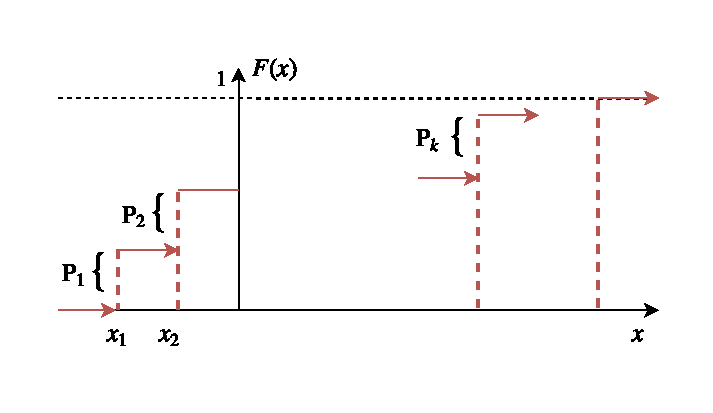
\includegraphics[width=\textwidth,height=\textheight,keepaspectratio]{Images/plot2-1.pdf}
	\end{center}
	\caption{Дискретный закон распределения вероятностей.}
\end{figure}

Такой набор чисел называется дискретным законом распределения вероятностей на вещественной прямой.
\begin{example}
	$\{ \Prob_k = \frac{1}{N} \}$ --- дискретный равномерный закон, $k = 1, \ldots, N$
\end{example}
\begin{example}
	$\{ p_1, p_2 \} : p_1 = 1 - p_2$ --- бернуллиевское дискретное распределение (часто обозначают как $p, q$).
\end{example}
\begin{example}
	${ \{ {\Prob}_{m}^{ (n) } \} }_{m = 0, 1, \ldots, n}$, $n$ --- число испытаний, $p$ --- вероятность появления успеха в каждом испытании. \\
	$\Prob_m^{(n)} = C_n^m \cdot p^m \cdot (1 - p)^{n-m}$ --- биномиальное дискретное распределение.
\end{example}
\begin{example}
	$\Prob_m = \frac{a^m}{m!} \cdot e^{-a}, a \in \mathbb{R}, a > 0, m = 0, 1, \ldots$ --- дискретный закон распределения Пуассона.
\end{example}
\subsubsection{Абсолютно непрерывные вероятностные меры}
Пусть $F(x)$ непрерывна $\forall x \in \mathbb{R}$, при этом существует вещественная неотрицательная кусочно-непрерывная функция плотности распределения вероятностей $f(x)$:
\[
	f(x) \geqslant 0 : F(x) = \int\limits_{-\infty}^x f(t) dt
\]
В этом случае
\[
	\Prob \{ (a, b] \} = \int\limits_a^b f(x) dx
\]
Очевидно, что если $x$ --- точка непрерывности $f(x)$, $x \in \mathbb{R}$, то
\[
	F'(x) = f(x)
\]

Плотностью распределения может быть любая кусочно-непрерывная, вещественнозначная функция $f(x)$, удовлетворяющая условию нормировки
\[
	\int\limits_{-\infty}^{+\infty} f(x) dx = 1
\]
\begin{example}
	Равномерное распределение на отрезке $[a, b]$, $a < b$
	\[
		f(x) = \frac{1}{b-a}, \; a \leqslant x \leqslant b
	\]
	Если $x < a$ или $x > b$, тогда
	\[
		f(x) = 0.
	\]
	Итак,
	\[
		f(x) =
		\begin{dcases*}
			\frac{1}{b-a}, \; a \leqslant x \leqslant b \\
			\;\;\;\;0, \; x < a \text{ или } x > b
		\end{dcases*}
	\]
\end{example}
\begin{example} Распределение Гаусса (нормальное)
	\[
		f(x) \sim N(a, \sigma), a \in \mathbb{R}, \sigma > 0
	\]
	Тогда
	\[
		f(x) = \underbrace{\frac{1}{\sqrt{2 \pi } \sigma}}_{\underset{\text{множитель}}{\text{норм.}}}\cdot e ^{-\frac{(x-a)^2}{2 \sigma^2}}
	\]
\end{example}
\begin{example} $\Gamma$-распределение \\
	Здесь в нормирующем множителе для плотности участвует $\Gamma$-функция
	\[
		f(x) =
		\begin{dcases*}
			\;\; 0, \; x \leqslant 0 \\
			\frac{\alpha^\lambda}{\Gamma(\lambda)} \cdot x^{\lambda - 1} \cdot e^{-\alpha x}, \; x > 0
		\end{dcases*}
	\]
	$\alpha$ --- параметр масштаба, $\lambda$ --- параметр формы. \\
	Экспоненциальное (показательное) распределение получаем при $\lambda = 1$:
	\[
		f(x) =
		\begin{cases}
			\alpha e^{-\alpha x}, \; x \geqslant 0 \\
			\;\;\; 0, \; x < 0
		\end{cases}
	\]
\end{example}
\subsubsection{Сингулярные вероятностные меры на $\mathbb{R}^1$}
Оказывается, $F(x)$ может быть непрерывной, но не иметь плотности. \\
$F(x)$ --- непрерывная функция распределения, функции плотности вероятности $f(x)$ не существует.
\begin{example} Канторова функция.
	\[
		F(x) =
		\begin{cases}
			0, x \leqslant 0 \\
			1, x \geqslant 1
		\end{cases}
	\]
	Представим, как ведёт себя функция распределения при $x \in (0, 1)$




	

	\begin{figure}[H]
	\begin{center}
	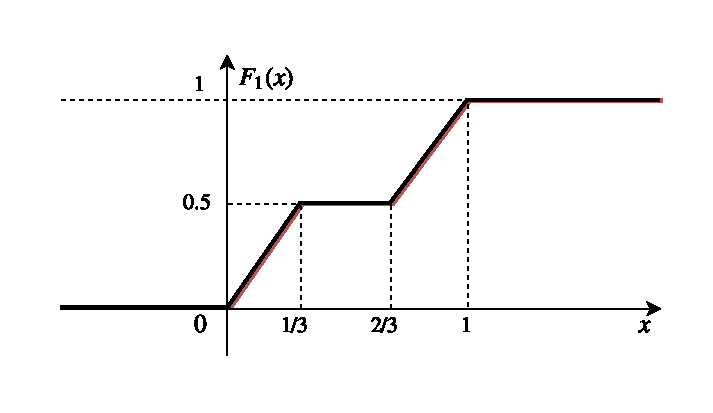
\includegraphics[width=\textwidth,height=\textheight,keepaspectratio]{Images/plot2-2.pdf}
	\end{center}
	\caption{$F_1(x)$ --- первое приближение Канторовой функции.}
	\end{figure}
	\begin{figure}[H]
	\begin{center}
	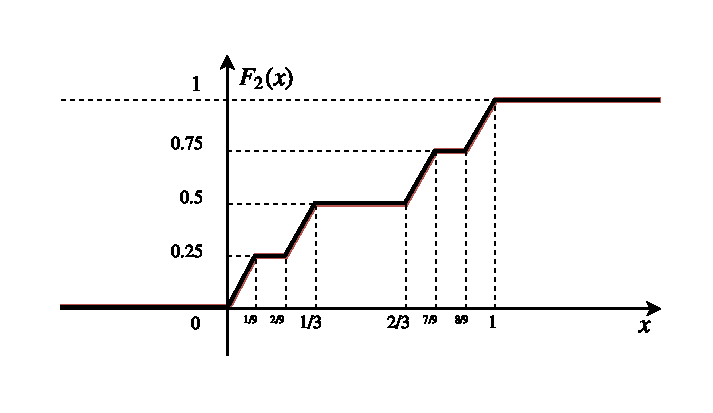
\includegraphics[width=\textwidth,height=\textheight,keepaspectratio]{Images/plot2-3.pdf}
	\end{center}
	\caption{$F_2(x)$ --- второе приближение Канторовой функции.}
	\end{figure}

	$F_n(x) \underset{n \to \infty}{\rightarrow} F(x)$ --- Канторова функция. \\
	Длина интервалов, на которой Канторова функция должна быть постоянна:
	\[
		\frac{1}{3} + \frac{2}{9} + \frac{4}{27} + \ldots = \frac{1}{3} \cdot \sum\limits_{n = 0}^\infty \left(\frac{2}{3}\right)^n = 1.
	\]
	$f(x)$ почти всюду обращается в 0, за исключением, может быть, множеств меры нуль. \\
	Функция называется сингулярной, поскольку она сингулярна по отношению к мере Лебега.
\end{example}
\begin{theorem} \textit{(Лебега)}.  
	Любая функция распределения в таком измеримом пространстве может быть представлена в виде:
	\[
		F(x) = p_1 F_1(x) + p_2 F_2(x) + p_3 F_3(x)
	\]
	где $p_i \geqslant 0, \sum\limits_{i=1}^3 p_i = 1$,
	\begin{itemize}
		\item $F_1 (x)$ --- дискретная функция распределения
		\item $F_2 (x)$ --- абсолютно непрерывная функция распределения
		\item $F_3 (x)$ --- сингулярная функция распределения
	\end{itemize}
\end{theorem}

\setcounter{equation}{0}
\section{Случайные величины}
\begin{definition}
	Вещественнозначная функция $\xi (\omega)$, определённая на измеримом пространстве $(\Omega, \mathcal{F})$, называется \textit{случайной величиной}, если
	\[
		\xi: \xi(\omega), \xi : \Omega \rightarrow \mathbb{R}^1
	\]
	\[
		\forall B \in \mathcal{B}(\mathbb{R}^1) \text{ --- борелевское множество из $\sigma$-алгебр $\mathcal{B}(\mathbb{R}^1)$}
	\]
	$\{ \omega : \xi(\omega) \in B \} \in \mathcal{F}$ --- такое множество всех элементов событий, для которых $\xi(\omega) \in B$ является событием.
	\begin{equation}
		\forall B : \xi^{-1}(B) = \{ \omega : \xi(\omega) \in B \} \in \mathcal{F}
	\end{equation}
\end{definition}
\begin{definition}
Вероятностная мера $\mathcal{P}_\xi$ на измеримом пространстве $(\mathbb{R}^1, \mathcal{B}(\mathbb{R}^1))$ такая, что:
\[
	\mathcal{P}_\xi (B) \overset{\textrm{def}}{=} \Prob \{ \omega : \xi (\omega) \in B \}
\]
называется \textit{распределением вероятностей случайной величины} $\xi$ на измеримом пространстве $(\mathbb{R}^1, \mathcal{B}(\mathbb{R}^1))$. \\
Эту вероятность далее будем обозначать как
\[
	\Prob \{ \xi \in B \}.
\]
\end{definition}
\begin{definition}
	$\forall x \in \mathbb{R}$ определим
	\[
		F_\xi (x) = \Prob \{ \omega : \xi (\omega) \leqslant x \} = \mathcal{P}_\xi \{ (-\infty, x] \}
	\]
	Здесь в качестве $B$ выступает интервал $(-\infty, x]$. \\
	$F_\xi (x)$ --- функция распределения случайной величины $\xi$. Обозначать далее будем как
	\[
		F_\xi (x) = \Prob \{ \xi \leqslant x \}
	\]
\end{definition}
Итак, каждая случайная величина порождает своё вероятностное пространство
\[
	\xi : \Omega \rightarrow \mathbb{R}^1 \rightarrow (\mathbb{R}^1, \mathcal{B}(\mathbb{R}^1), \mathcal{P}_\xi)
\]
Оказывается, множество пробных борелевских множеств можно существенно сузить, так как для определения вероятности достаточно задать вероятности интервалов. \\
Следовательно, функция распределения случайной величины полностью определяет распределение случайной величины. По $F_\xi (x)$ можно восстановить меру борелевского множества.\\
Рассмотрим типы случайных величин.
\begin{enumerate}
	\item Если возможные значения случайной величины образуют не более чем счётное множество, то такая случайная величина называется \textit{дискретной} случайной величиной. \\
	$\xi$ -- дискретна, $\{x_j \text{ --- возможное значение} \}_{j = 1, 2, \ldots}$, $\Prob \{ \xi = x_i \} = p_i$ --- вероятности. \\
	Можно вычислить все вероятности, связанные с $\xi$. $B$ -- борелевское множество, $B \in \mathcal{B} (\mathbb{R}^1)$, тогда
	\[
		\mathcal{P}_\xi (B) = \Prob \{ \xi \in B\} = \Prob \left(\sum\limits_{j : x_j \in B} (\xi = x_j)\right) = \sum\limits_{j : x_j \in B} \underset{p_j}{\Prob (\xi = x_j)}
	\]
	В этом случае
	\[
		F_\xi (x) = \sum\limits_{j : x_j \leqslant x} p_j \text{ --- ст. функция с разрывами в $x_j$}
	\]
	\item Случайная величина называется \textit{непрерывной}, если
	\[
		\exists f_\xi (x) \geqslant 0 : F_\xi (x) = \int\limits_{-\infty}^x f_\xi (t) dt
	\]
	\item Случайная величина называется \textit{сингулярной}, если функция её распределения $F_\xi (x)$ непрерывна, но функция плотности вероятности $f_\xi (x)$ не существует.
\end{enumerate}
Заметим, что в то время как любая случайная величина однозначно определяет свою функцию распределения, существует сколько угодно различных случайных величин, имеющих одну и ту же функцию распределения.
\begin{example} $x_i: -1, +1$; $p_i: \frac{1}{2}, \frac{1}{2}$; $\xi_i - \xi = \eta$

\begin{figure}[H]
	\begin{center}
	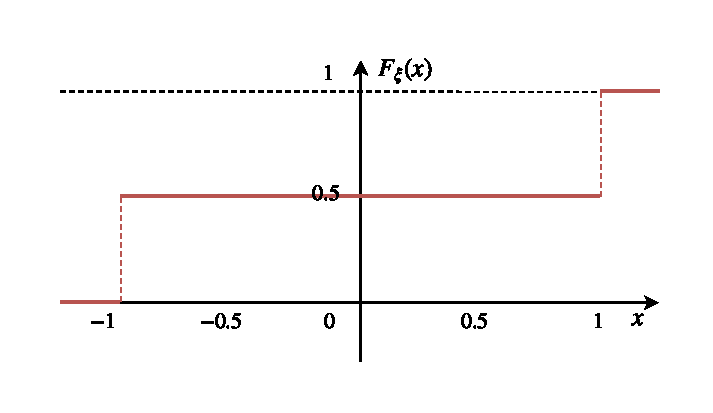
\includegraphics[width=\textwidth,height=\textheight,keepaspectratio]{Images/plot2-4.pdf}
	\end{center}
	\caption{Пример функции распределения.}
\end{figure}

	\[
		F_\eta = F_\xi =
		\begin{dcases*}
			0, \; x < -1 \\
			\frac{1}{2}, \; -1 \leqslant x < 1 \\
			1, \; x \geqslant 1
		\end{dcases*}
	\]
\end{example}
\begin{definition}
	Вещественнозначная функция $g(x)$, $x \in \mathbb{R}$ называется \textit{борелевской}, если для любого борелевского множества при отображении $g$ его полный прообраз также является борелевским множеством
	\[
		g : \mathbb{R}^1 \rightarrow \mathbb{R}^1, B \in \mathcal{B} (\mathbb{R}^1), g^{-1} (B) = \{ x, x \in \mathbb{R}^1 : g(x) \in B \}
	\]
\end{definition}
\begin{theorem}
	Пусть $\xi (\omega)$ --- случайная величина.
	\[
		\xi (\omega) : \Omega \rightarrow \mathbb{R}^1
	\]
	\[
		g(x) : \mathbb{R}^1 \rightarrow \mathbb{R}^1 \text{ --- борелевская функция}
	\]
	$\Omega = \{ \omega \}$ --- значение элементарного события. Тогда $\eta (\omega) = g (\xi (\omega))$ является случайной величиной.
\end{theorem}
\begin{proof}
	$B \in \mathcal{B} (\mathbb{R}^1)$
	\[
			\{ \omega : \eta (\omega) \in B \} = \{ \omega : g(\xi(\omega)) \in B \} = \{ \omega : \xi(\omega) \in g^{-1} (B) \} \in \mathcal {F}
	\]
	\[
		\xi \sim (\Omega, \mathcal{F})
	\]
	Это означает, что $\eta(\omega)$ --- случайная величина.
\end{proof}
Также возможно конструировать случайные величины как функции других случайных величин.
\subsection{Примеры случайных величин}
\begin{itemize}
	\item Пусть $A$ --- событие, $\xi(\omega) \equiv I_A (\omega) = \begin{cases}
		1, \omega \in A \\
		0, \omega \not \in A
	\end{cases} $ \\
	Задана функция-индикатор.
	\item Пусть испытание --- бросание игральной кости. Случайная величина --- число выпавших на верхней грани очков, всего возможно 6 значений, вероятность каждого -- $\frac{1}{6}$. Можем задать дискретное распределение с параметром 6.
	\item Распределение последовательности испытаний Бернулли. Пусть $\xi_i (\omega)$ --- число появления «успеха» в $i$-ом испытании.
%TODO: fix formatting
	\[
		\xi_i (\omega) : I_{A_i} (\omega) = \begin{cases}
		1, \omega \in A_i \\
		0, \omega \not \in A_i
	\end{cases} \text{--- Бернуллиевская случайная величина}
	\]
	Пусть $A_i$ --- в $i$-ом испытании «успех».
	\item Рассмотрим серию из $n$ испытаний Бернулли. $\mu_n$ --- число появления «успеха» в серии из $n$ испытаний. Пусть $p$ --- вероятность появления успеха в каждом из испытаний.
	\[
		{\{ \Prob \{ \mu_n = m \} = C_n^m p^m (1-p)^{n-m} \}}_{m = 0, \ldots, n}
	\]
	\item Пусть испытание --- «бросание» точки в отрезок случайным образом. $\Omega = \{ \omega \}$.
	\[
		\begin{cases}
			\Omega = [a, b] \text{ $a < b$ } \\
			\mathcal{F}
		\end{cases}
	\]
	\[
		\xi (\omega) = \omega
	\]
	\[
		F_\xi (x) \overset{\textrm{def}}{=} \Prob \{ \xi \leqslant x \} = \frac{x - a}{b - a}, \; a \leqslant x \leqslant b, \; \xi \in [a, x]
	\]
	\[
		F' (x) = \frac{1}{b-a}, x \in [a, b]
	\]
	\[
		x < a : \mathcal{F}_\xi (x) = 0, \; x > b : \mathcal{F}_\xi (x) = 1
	\]
\begin{figure}[H]
	\begin{center}
	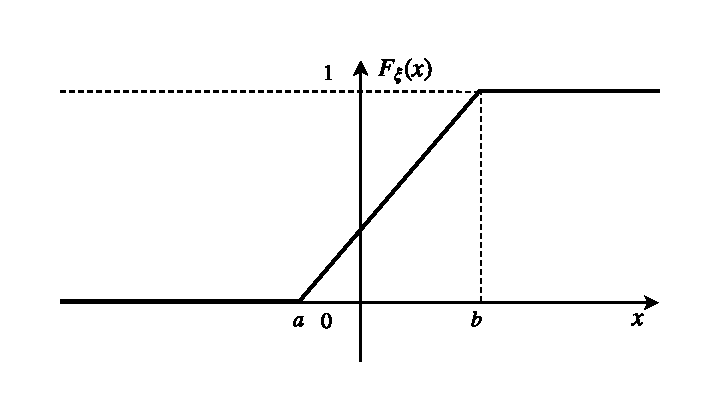
\includegraphics[width=\textwidth,height=\textheight,keepaspectratio]{Images/plot2-5.pdf}
	\end{center}
	\caption{Пример распределения случайной величины.}
\end{figure}
\end{itemize}
\setcounter{equation}{0}
\section{Способы задания вероятности на измеримом пространстве $(\mathbb{R}^n, \mathcal{B} (\mathbb{R}^n))$}
$\mathbb{R}^1 \times \ldots \times \mathbb{R}^1$ --- $\mathbb{R}^n$ --- прямое произведение $n$ экземпляров вещественных прямых.
\[
	\{ x = \{ x_1, \ldots, x_n \} \}, \forall i: -\infty < x_i < +\infty
\]
Определим пространство элементарных событий. Определим прямоугольник (объект) в $\mathbb{R}^n$.
\[
	-\infty \leqslant a_k < b_k < +\infty, \; k = 1, \ldots, n
\]
\[
	(a_1, b_1] \times \ldots \times (a_k, b_k] \times \ldots \times (a_n, b_n]
\]
\[
	B_1 \times \ldots \times B_n, B_i \in \mathcal{B} (\mathbb{R}^1)
\]
\[
	\sigma \{ (B_1 \times \ldots \times B_n) \} = \mathcal{B} (\mathbb{R}^n)
\]
Построим вероятностное пространство на этом измеримом пространстве. Пусть $\Prob$ --- вероятностная мера на $(\mathbb{R}^n, \mathcal{B}(\mathbb{R}^n))$. \\
Рассмотрим функцию $n$-мерной точки $F : \mathbb{R}^n \rightarrow \mathbb{R}^1$
\begin{equation}
	F (x_1, \ldots, x_n) = \Prob \{ (-\infty, x_1] \times \ldots \times (-\infty, x_n] \}
\end{equation}
Введём разностный оператор.
\[ \Delta_{a_i b_i} F(x_1, \ldots, x_n) = F(x_1, \ldots, x_{i-1}, b_i, x_{i+1}, \ldots, x_n) - \]
\[ - F(x_1, \ldots, x_{i-1}, a_i, x_{i+1}, \ldots, x_n), \; a_i < b_i, \; i = 1, \ldots, n. \]
\begin{example}
	$\Delta_{a_1 b_1} \Delta_{a_2 b_2} \ldots \Delta_{a_n b_n} F(x_1, \ldots, x_n) = \Prob \{(a_1, b_1] \times \ldots \times (a_n, b_n] \}$
	%TODO: ex
\end{example}
Отметим определяющие свойства функции $F$.
\begin{enumerate}
	\item $\forall k :$ $-\infty \leqslant a_k < b_k < +\infty$, $k = 1, \ldots, n$
	\[
		\Delta_{a_1 b_1} \cdot \ldots \cdot \Delta_{a_n b_n} F(x_1, \ldots, x_n) \geqslant 0
	\]
	\item Из монотонности вероятности --- $F$ монотонно не убывает по любому своему аргументу \\
	Из непрерывности вероятности --- $F$ непрерывна справа по совокупности аргументов в каждой точке.
	\[
		x, x^{(k)} \in \mathbb{R}^n \Rightarrow F(x^{(k)}) \underset{k \to \infty}{\rightarrow}  F(x) 
	\]
	\item Устремим каждый аргумент функции к $+\infty$:
	\[
		F(+\infty, \ldots, +\infty) = 1
	\]
	\item $\lim\limits_{x \downarrow y} F (x_1, \ldots, x_n) = 0$, $y \in \mathbb{R}^n$, $y_i = -\infty$.
\end{enumerate}
\begin{definition}
	Любую функцию $n$ аргументов, удовлетворяющую условиям (1, 2, 3, 4), будем называть \textit{функцией распределения} в $\mathbb{R}^n$
\end{definition}
\begin{example}
	$n = 2$ \\
	\[
		F(x_1, x_2) =
		\begin{cases}
			0, \; x_1 + x_2 < 1 \\
			1, \; x_1 + x_2 \geqslant 1
		\end{cases}
	\]
	%TODO: упражнение --- доказать 2, 3, 4
	Очевидно, свойства (2, 3, 4) выполнены. Применим разностный оператор.
	\[
		a_1 = 0, \; b_1 = 1 : \Delta_{a_1 b_1} F(x_1, x_2) = F(1,x_2) - F(0, x_2)
	\]
	\[ a_2 = 0, \; b_2 = 1 : \Delta_{a_2 b_2} [\Delta_{a_1 b_1} F(x_1, x_2)] = [F(1,1) - F(0, 1)] - \]
	\[ [F(1,0) - F(0,0)] = 1 - 1 - 1 + 0 = -1 \]
	Условие (1) не выполнено.
\end{example}
\begin{theorem}
	Пусть $F = F(x_1, \ldots, x_n)$ --- функция распределения на $\mathbb{R}^n$. Тогда на вероятностном пространстве $(\mathbb{R}^n, \mathcal{B}(\mathbb{R}^n))$ существует единственная вероятностная мера $\Prob$:
	\begin{equation}
		\Prob \{ (a_1, b_1] \times \ldots \times (a_n, b_n] \} = \Delta_{a_1 b_1} \dots \Delta_{a_n b_n} F(x_1, \ldots, x_n)
	\end{equation}
\end{theorem}
%TODO: ссылки на выражения 1,2; фикс нумераций выражений
(1) и (2) говорят о том, что между вероятностью и функцией распределения в $\mathbb{R}^n$ установлено взаимно однозначное соответствие.

\section{Случайный вектор и его распределение на измеримом пространстве $(\mathbb{R}^n, \mathcal{B}(\mathbb{R}^n))$}
\begin{definition}
	Любой упорядоченный набор случайных величин $\xi_1, \ldots, \xi_n$, заданный на $(\Omega, \mathcal{F}, \Prob)$, называется случайным вектором.
	\[
		\overline{\xi} = (\xi_1, \ldots, x_n)
	\]
	Если для любого $B \in \mathcal{B}(\mathbb{R}^n)$
	\[
		\{ \omega: \xi (w) \in B \} \in \mathcal{F} \text{ --- событие, то $\overline{\xi}$ --- случайный вектор.}
	\]
	\[
		B = B_1 \times \ldots \times B_n, B_i \in \mathcal{B} (\mathbb{R}^1)
	\]
	\[
		\{ \omega : \xi_1 (\omega) \in B_1, \ldots, \xi_n (\omega) \in B_n \}
	\]
\end{definition}
\begin{definition}
	Распределением вероятностей $n$-мерного случайного вектора называется функция множества $\mathcal{P}_{\overline{\xi}} (B)$ такая, что
	\[
		B \in \mathcal{B} (\mathbb{R}^n) : \mathcal{P}_{\overline{\xi}} \overset{\textrm{def}}{=} \Prob \{ \omega : \overline{\xi} (\omega) \in B \}
	\]
\end{definition}
\begin{definition}
	Функцией распределения случайного вектора $\overline{\xi}$ называется функция $n$-мерной точки
	\[
		F_{\overline{\xi}} (x_1, \ldots, x_n) \overset{\textrm{def}}{=} \Prob \{\omega : \xi_1 (\omega) \leqslant x_1, \ldots, \xi_n (\omega) \leqslant x_n \}
	\]
	\[
		B \in \mathcal{B} (\mathbb{R}^n) : \mathcal{P}_{\overline{\xi}} \overset{\textrm{def}}{=} \Prob \{ \omega : \overline{\xi} (\omega) \in B \} \equiv \Prob \{ \overline{\xi} (\omega) \}
	\]
\end{definition}
Отметим свойство согласованности функции распределения случайного вида.
\begin{enumerate}
	\item $\lim\limits_{x_n \to +\infty} F_{\xi_1, \ldots, \xi_n} (x_1, \ldots, x_n) = F_{\xi_1, \ldots, \xi_{n-1}} (x_1, \ldots, x_{n-1})$
	\item $\lim\limits_{x_n \to -\infty} F_{\xi_1, \ldots, \xi_n} (x_1, \ldots, x_n) = 0$
\end{enumerate}
Пусть
\[
 (:) (\xi_{i_1}, \ldots, \xi_{i_k}), 1 \leqslant i_1 < \ldots < i_k \leqslant n; \text{ $k < n$ --- подвектор}
\]
\begin{lemma}
	Распределение любого подвектора исходного вектора (:) полностью определяется распределением исходного вектора $\overline{\xi}$.
	$\overline{\eta} = (\xi_1, \ldots, \xi_k), k < n$ порождает на $(\mathbb{R}^k, \mathcal{B}(\mathbb{R}^k))$ вероятностную меру $\mathcal{P}_{\overline{\eta}}$. $B \in \mathcal{B}(\mathbb{R}^k)$.
\[
		\mathcal{P}_{\overline{\eta}}(B) \overset{\textrm{def}}{=} \Prob(\overline{\eta} \in B) = \Prob ((\xi_1, \ldots, \xi_k) \in B) =
\]
\[
	\Prob \{(\xi_1, \ldots, \xi_k) \in B, (\xi_{k+1}, \ldots, \xi_n) \in \mathbb{R}^{n-k} \} =
\]
\[
	 = \Prob \{(\xi_1, \ldots, \xi_n) \in B \times \mathbb{R}^{n-k} = \mathcal{P}_{\overline{\xi}} (B \times \mathbb{R}^{n-k})
\]
Обратное не верно.
\end{lemma}
Случайный $n$-мерный вектор имеет дискретное распределение вероятностей, если он может принимать не более чем счётное число возможных значений.
\[
	\overline{\xi} = (\xi_1, \ldots, \xi_n), x^{(j)} = (x_1^{(j)}, \ldots, x_n^{(j)}), \Prob \{ \overline{\xi} = x^{(j)} \} = p_j, \sum\limits_{j=1}^n p_j = 1
\]
\[
		\mathcal{P}_{\overline{\xi}} (B) = \Prob (\overline{\xi} \in B) = \sum\limits_{j: x^{(j)} \in B} p_j =
\]
\[
	= \sum\limits_{j: x_1^{(j)} \in B} \ldots \sum\limits_{j: x_n^{(j)} \in B} \Prob (\xi_1 = x_1^{(j)}, \ldots, \xi_n = x_n^{(j)})
\]
\[ 
F_{\overline{\xi}} (x_1, \ldots, x_n) = \Prob \{ \xi_1  \leqslant x_1, \ldots, \xi_n \leqslant x_n) = \]
\[ = \sum\limits_{j: x_1^{(j)} \leqslant x_1} \ldots \sum\limits_{j: x_n^{(j)} \leqslant x_n} \Prob (\xi_1 = x_1^{(j)}, \ldots, \xi_n = x_n^{(j)})
\]
Будем говорить, что $n$-мерный случайный вектор имеет абсолютно непрерывное распределение, если существует функция плотности вероятности $f_{\overline{\xi}} (x_1, \ldots, x_n) \geqslant 0, \int\limits_{\mathbb{R}^n} f_{\overline{\xi}} (x) dx = 1$, такая, что
\[
	\mathcal{P}_{\overline{\xi}} (B) \overset{\textrm{def}}{=} \Prob (\overline{\xi} \in B) = \int\limits_B f_{\overline{\xi}} (x) dx, B \in \mathcal{B} (\mathbb{R}^n)
\]
\begin{example}
	$S \in \mathbb{R}^n$. \\
	\[
		f_{\overline{\xi}} (x) = \begin{dcases*}
 		\frac{1}{|S|}, x \in S \\
 		\;\; 0, x \not \in S
 		\end{dcases*}
	\]
	Тогда
	\[
		\mathcal{P}_{\overline{\xi}} = \Prob \{ \xi \in B \} = \frac{|B \cap S|}{|S|}
	\]
	Рассмотрим положительно определённую симметричную матрицу $R$
	\[
		R = {\{ r_{ij} \}}_{\underset{j = 1, \ldots, n}{i = 1, \ldots, n}}, r_{ij} = r_{ji}
		\]
	\[
		\forall x_i, x_j \in \mathbb{R}^1: \sum\limits_{i, j = 1}^n r_{ij} \cdot x_i \cdot x_j > 0
	\]
	\[
		det R > 0 \Rightarrow \exists R^{-1} = B = {\{ b_{ij} \}}_{\underset{j = 1, \ldots, n}{i = 1, \ldots, n}}
	\]
	$n$-мерная невырожденная функция плотности вероятности:
	\[
		f (x_1, \ldots, x_n) = \frac{{[det B]}^{\frac{1}{2}}}{2 \pi^{\frac{n}{2}}} = e^{-\frac{1}{2} b_{ij}(x_i - a_i)(x_j - a_j)}, a_i, a_j \in \mathbb{R}^1
	\]
\end{example}

\setcounter{equation}{0}
\section{Независимость случайных величин}
Пусть имеется упорядоченный набор случайных величин $\xi_1, \ldots, \xi_n$, заданный на вероятностном пространстве $(\Omega, \mathcal{F}, \Prob)$.
\begin{definition}
	Будем говорить, что $\xi_1, \ldots, \xi_n$ независимы, если для любого набора одномерных борелевских множеств $\{ B_1, \ldots, B_n \}, B_i \in \mathcal{B}(\mathbb{R}^1)$ выполняется:
	\begin{equation}
		\Prob \{ \xi_1 \in B_1, \ldots, \xi_n \in B_n \} = \prod\limits_{i = 1}^n \underbrace{\Prob \{ \xi_i \in B_i \}}_{\mathcal{P}_{\xi_i}(B_i)}
	\end{equation}
	\[
		\mathcal{P}_{\overline{\xi}} (B_1 \times \ldots \times B_n), B_i = (-\infty, x_i]
	\]
	\begin{equation}
		\forall x: F_{\xi_1, \ldots, \xi_n} (x_1, \ldots, x_n) = F_{\xi_1} (x_1) \cdot \ldots \cdot F_{\xi_n} (x_n)
	\end{equation}
	\begin{equation}
		\underbrace{\Delta_{a_1 b_1} \ldots \Delta_{a_n b_n} (F_{\xi_1, \ldots, \xi_n} (x_1, \ldots, x_n))}_{\mathcal{P}_{ \overline{\xi}} \{ (a_1, b_1] \times \ldots \times (a_n, b_n] \} } =
		\prod\limits_{i = 1}^n \underbrace{ \Delta_{a_i b_i} F_{\xi_i} (x_i) }_{\mathcal{P}_{\xi_i} \{ (a_i, b_i] \}}
	\end{equation}
	(1), (2), (3) эквивалентны.
\end{definition}

\begin{theorem}
	Пусть имеется набор дискретных случайных величин $\xi_1, \ldots, \xi_n$. Они независимы тогда и только тогда, когда
	\[
		\Prob \{ \xi_1 = x_1, \ldots, \xi_n = x_n \} = \prod\limits_{i = 1}^n \Prob \{ \xi_i = x_i \}, \forall {\{ x^{(j)} \}}_{j = 1, 2, \ldots}
	\]
\end{theorem}

\begin{theorem}
	Пусть имеется набор абсолютно непрерывных случайных величин $\xi_1, \ldots, \xi_n$. Они независимы тогда и только тогда, когда
	\[
		f_{\xi_1, \ldots, \xi_n} (x_1, \ldots, x_n) = \prod\limits_{i = 1}^n f_{\xi_i} (x_i), x \in \mathbb{R}^n
	\]
\end{theorem}

\begin{addition}
	Пусть имеется набор случайных величин $\xi_1, \ldots, \xi_n$, $g_1 (x), \ldots, g_n(x)$ --- набор борелевских функций, $x \in \mathbb{R}^1$. Тогда $g_1(\xi_1), \ldots, g_n (\xi_n)$ также независимы.
\end{addition}

\begin{interjection}
	Сконструируем интеграл Лебега. Пусть имеется измеримое пространство $[a, b]$, $g(x) = y$ --- непрерывная ограниченная функция.
	\begin{itemize}
		\item $A$ --- точка верхней границы $g(x)$,
		\item $B$ --- точка нижней границы $g(x)$.
	\end{itemize}
	\[
		A = y_0 < y_1 < \ldots < y_n = B
	\]
	\[
		S_i = \{ x \}: y_{i - 1} < g(x) < y_i, x \in [a, b]
	\]
	Тогда
	\[
		\lim\limits_{max(y_i - y_{i - 1}) \to 0} \sum\limits_{i = 1}^n y_i \mu (S_i) \overset{\textrm{def}}{=} \int\limits_a^b g(x) dx
	\]
\end{interjection}

\begin{addition}
	Конструкция интеграла Лебега не зависит от того, на каком измеримом пространстве он задаётся, в отличие от интеграла Римана, не определяющемся на абстрактном пространстве $(\Omega, \mathcal{F})$. \\
	В конструкции Лебега (когда $\Omega$ --- отрезок вещественной прямой) точки функции группируются согласно близости значений самой функции, а не как в интеграле Римана по близости на самой оси. \\
	Таким образом, интегральные суммы Римана будут иметь предел для не слишком разрывных функций. Интеграл Лебега имеет смысл для более широкого класса функций. \\
	Пусть интеграл Римана существует в смысле абсолютной сходимости, значит, совпадает с интегралом Лебега. \\
	Для любого не более чем счётного набора попарно несовместных событий $B_1, \ldots, B_n, \ldots$ интеграл Лебега:
	\[
		\int\limits_{\sum\limits_i B_i} = \sum\limits_i \int\limits_{B_i} \ldots
	\]
\end{addition}

\begin{theorem}
	\textit{(Фубини)}. Рассмотрим специальный класс измеримых пространств с определённой на них вероятностной мерой: $(\Omega, \mathcal{F}, \Prob)$. Пусть $\Omega_1 = \{ \omega_1 \}$, $\Omega_2 = \{ \omega_2 \}$
	\[
		\Omega = \Omega_1 \times \Omega_2, \mathcal{F} = \mathcal{F}_1 \times \mathcal{F}_2, \Prob = \Prob_1 \times \Prob_2
	\]
	\[
		A \in \mathcal{F}_1, B \in \mathcal{F}_2, A \times B \in \mathcal{F}
	\]
	\[
		\Prob (A \times B) = \Prob_1 \times \Prob_2 (A \times B) = \Prob_1 (A) \times \Prob_2 (B)
	\]
	Тогда, если
	\[
		\iint\limits_{\Omega_1 \times \Omega_2} | \xi (\omega_1, \omega_2) | d (\Prob_1 \times \Prob_2) < +\infty \text{ --- интеграл конечен}
	\]
	То
	\[
		\exists \int\limits_{\Omega_i} \xi (\omega_1, \omega_2) d \Prob_i, \; i = 1, 2
	\]
	\[
		\iint\limits_{\Omega_1 \times \Omega_2} \xi(\omega_1, \omega_2) d (\Prob_1 \times \Prob_2) = \int\limits_{\Omega_1} \left[\int\limits_{\Omega_2} \xi (\omega_1, \omega_2) d \Prob_2 \right] d \Prob_1 =
	\]
	\[
		= \int\limits_{\Omega_2} \left[\int\limits_{\Omega_1} \xi(\omega_1, \omega_2) d \Prob_1 \right] d \Prob_2
	\]
\end{theorem}
\begin{example}
	$n = 2.$
	\[
		(\xi, \eta), (\mathbb{R}^2, \mathcal{B} (\mathbb{R}^2), \mathcal{P}_{\xi, \eta}), f_{\xi, \eta} (x, y)
	\]
	\begin{itemize}
		\item $\xi \sim x$ --- возможное значение $\xi$
		\item $\eta \sim y$ --- возможное значение $\eta$
	\end{itemize}
	Пусть $B \in \mathcal{B} (\mathbb{R}^2)$
	\[
		\mathcal{P}_{\xi, \eta} (B) = \Prob \{ (\xi, \eta) \in B \} = \iint\limits_B f_{\xi, \eta} (x, y) dx dy
	\]
	\[
		f_{\xi} (x) = \int\limits_{-\infty}^{+\infty} f_{\xi, \eta} (x, y) dy, \; f_{\eta} (y) = \int\limits_{-\infty}^{+\infty} f_{\xi, \eta} (x, y) dx
	\]
	Выведем $f_{\xi} (x)$. Пусть $B_1 \in \mathcal{B}(\mathbb{R}^1)$,
	\[
		\mathcal{P}_{\xi} (B) = \Prob \{ \xi \in B \} = \Prob \{ (\xi, \eta) \in B \times \mathbb{R}^1 \} =
	\]
	\[
		\iint\limits_{B \times \mathbb{R}^1} f_{\xi, \eta} (x, y) dx dy \overset{\text{(т. Фубини)}}{=} \int\limits_{B_1} \left[ \int\limits_{\mathbb{R}^1} f_{\xi, \eta} (x, y) dy \right] dx
	\]
	Для $f_{\eta} (x)$ вывод аналогичен.
\end{example}


\newpage
\setcounter{section}{0}
\chapter{Числовые характеристики распределения случайных величин}
\setcounter{equation}{0}
\section{Математическое ожидание случайной величины}
\begin{definition}
  Математическим ожиданием случайной величины $\xi$ на вероятностном пространстве $(\Omega, \mathcal{F}, \Prob)$ будем называть интеграл Лебега:
  \[
    \MExpect_{\xi} = \int\limits_{\Omega} \xi(\omega) d \Prob(\omega), \text{ при этом, если } \int\limits_{\Omega} | \xi(\omega) | d \Prob < +\infty
  \]
  T.e. если интеграл конечен. Иначе случайная величина математического ожидания не имеет.
  \[
    \exists \MExpect_{\xi} \Leftrightarrow \MExpect_{|\xi|} < +\infty
  \]
  \[
    \exists \MExpect_{\xi} \Rightarrow \forall A \in \mathcal{F} \;\;\exists \int\limits_A \xi(\omega) d \Prob = \int\limits_{\Omega} \xi \cdot I_A d \Prob = \MExpect \left[ \xi \cdot I_A \right]
  \]
  \[
    \MExpect I_A = \int\limits_{\Omega} I_A (\omega) d \Prob = \int\limits_A d \Prob = \Prob(A)
  \]
\end{definition}
\subsection{Свойства математического ожидания}
\begin{enumerate}
  \item Пусть $a, b$ --- константы. Тогда $\MExpect_a = a, \MExpect \left[ b \cdot \xi \right] = b \cdot \MExpect_{\xi}$
  \item $|\MExpect_{\xi}| \leqslant \MExpect_{|\xi|}$
  \item $\MExpect \left[ \xi + \eta \right] = \MExpect_{\xi} + \MExpect_{\eta}$
  \item $\forall \varepsilon > 0 : |\xi| \leqslant \varepsilon \Rightarrow |\MExpect_{\xi}| \leqslant \varepsilon$
  \begin{proof} \textit{(Свойство 4)}
    \[
      |\MExpect_{\xi}| \leqslant \MExpect_{|\xi|} = \int\limits_{\Omega} |\xi| d \Prob \leqslant \varepsilon \int\limits_{\Omega} d \Prob = \varepsilon \cdot \Prob(\Omega) = \varepsilon
    \]
  \end{proof}
  \item \textbf{Неравенство Чебышёва.} Пусть $\xi \geqslant 0$ --- случайная величина, $t > 0$, $t \in \mathbb{R}^1$. Тогда
  \[
    \Prob \{ \xi \geqslant t \} \leqslant \frac{\MExpect \xi}{t}
  \]
  Рассмотрим
  \[
    \Prob \{ \xi \geqslant t \} = \int\limits_{\{ \omega: \xi(\omega) \geqslant t\}} d \Prob \leqslant \int\limits_{\{ \xi \geqslant t \}} \frac{\xi(\omega)}{t} d \Prob \leqslant \frac{1}{t} \int\limits_{\Omega} \xi(\Omega) d \Prob = \frac{\MExpect \xi}{t}
  \]
\end{enumerate}
\begin{conclusion}
  $g(x)$ --- борелевская функция, $x \in (0, +\infty)$. $g(x)$ монотонно возрастает, $g(x) \geqslant 0$, $\xi$ --- случайная величина. $t > 0: g(t) \not= 0$
  \[
    \Prob \{ |\xi| \geqslant t \} \leqslant \frac{\MExpect [g(|\xi|)]}{g(t)}
  \]
  \[
    \Prob \{ |\xi| \geqslant t \} = \Prob \{ g(|\xi|) \geqslant g(t) \} \leqslant \frac{\MExpect g(|\xi|)}{g(t)}
  \]
  Пусть $g(x) = x^2$. $x \in (0, +\infty)$:
  \[
    \Prob \{ |\xi| \leqslant t \} \leqslant \frac{\MExpect \xi^2}{t^2}, t > 0
  \]
  \[
    g(x_1, \ldots, x_n), \; g: \mathbb{R}^n \to \mathbb{R}^1
  \]
  \[
    \forall B \in \mathcal{B} (\mathbb{R}^1) : g^{-1}(B) \in \mathcal{B} (\mathbb{R}^n)
  \]
  \[
    g^{-1} (B) = \{ x, x \in \mathbb{R}^n : g(x) \in B \}
  \]
  \[
    \overline{\xi} = (\xi_1, \ldots, \xi_n), g(\overline{\xi}) : \Omega \to \mathbb{R}^1, \xi_i: \Omega \to \mathbb{R}^n
  \]
\end{conclusion}
\begin{theorem} \textit{(О вычислении математического ожидания случайной величины.)} Пусть задан вектор случайных величин $\overline{\xi} = (\xi_1, \ldots, \xi_n)$ на вероятностном пространстве $(\Omega, \mathcal{F}, \mathcal{P})$. \\
$g(x) : \mathbb{R}^n \to \mathbb{R}^1$, $x \in \mathbb{R}^n$, $g$ --- борелевская функция. Тогда на конкретном вероятностном пространстве задан интеграл Лебега
\[
  \MExpect g(\overline\xi) = \int\limits_{\mathbb{R}^n} g(x) d \mathcal{P}_{\overline{\xi}} (x),\; x \in \mathbb{R}^n
\]
По определению математического ожидания задан также интеграл Лебега, но на абстрактном пространстве элементарных событий.
\[
  \int\limits_{\Omega} g (\overline{\xi}(\omega)) d \Prob (\omega)
\]
Мы понимаем равенство следующим образом: если первый интеграл существует, то второй интеграл так же существует и ему равен.
\end{theorem}
\begin{conclusion}
  Пусть задан дискретный вектор случайных величин $\overline{\xi} = (\xi_1, \ldots, \xi_n)$, возможные значения --- ${\{ x^{(j)} \}}_{j = 1, 2, \ldots} $,
  $g : \mathbb{R}^n \to \mathbb{R}^1$ --- борелевская функция. Тогда математическое ожидание
  \[
    \MExpect g(\overline{\xi}) = \sum\limits_{x^{(j)} \in {\{ x^{(i)} \}}_{i = 1, 2, \ldots}} g(x^{(j)}) \cdot \Prob \{ \overline{\xi} = x^{(j)} \}
  \]
  \[
    \MExpect_{\xi} = \sum\limits_j x_j \cdot \Prob \{ \xi = x_j \}
  \]
\end{conclusion}
\begin{conclusion}
  Пусть задан абсолютно непрерывный вектор случайных величин $\overline{\xi} = (\xi_1, \ldots, \xi_n)$, $f_{\overline{\xi}}(\underbrace{x_1, \ldots, x_n}_{x}), x \in \mathbb{R}^n$, $g$ --- борелевская функция. Определим:
  \[
    \MExpect g(\overline{\xi}) = \int\limits_{\mathbb{R}^n} g(x) f_{\overline{\xi}} (x) dx
  \]
  \[
    \MExpect_{\xi} = \int\limits_{-\infty}^{+\infty} x \cdot f_{\xi} (x) dx
  \]
\end{conclusion}
\begin{example} \textit{Равномерное распределение.}
  $\xi \sim U [a, b]$.
  \[
    f_{\xi} (x) = \begin{dcases*}
    \frac{1}{b-a},\; x \in [a, b] \\
    0,\; x \not\in [a, b]
  \end{dcases*}
  \]
  \[
    \MExpect_{\xi} = \int\limits_a^b \frac{x}{b-a} dx = \frac{a+b}{2}
  \]
\end{example}
\begin{example} \textit{Дискретная случайная величина (бернуллиевская), задающая некоторые распределение.}
  \[
    q = 0,\; p = 1;\; p + q = 1,\; \MExpect_{\xi} = p
  \]
  Рассмотрим биномиальную случайную величину. Пусть $\mu_n$ --- число появления <<успеха>> в $n$ испытаниях Бернулли. Также пусть $\xi_k$ --- число появления успеха в $k$-ом испытании Бернулли
  \[
    \mu_n = \sum\limits_{k = 1}^n \xi_k
  \]
  \[
    \MExpect_{\mu_n} = \MExpect \left[ \sum\limits_{k = 1}^n  \xi_k \right] = \sum\limits_{k = 1}^n \MExpect_{\xi_k} = np
  \]
\end{example}
\begin{example} \textit{Распределение вероятностей случайных величин Пуассона.} $\xi \sim \Prob [a], a > 0$
  \[
    \MExpect_{\xi} = \sum\limits_{k = 0}^{\infty} k \cdot \frac{a^k}{k \ !} e^{-a} = a \cdot e^{-a} \sum\limits_{k = 0}^{\infty} \frac{a^{k-1}}{(k-1) \ !} = a
  \]
\end{example}
\begin{example} \textit{Распределение вероятностей случайных величин Коши.}
  $a > 0$
  \[
    f_{\xi} (x) = \frac{a}{\pi (x^2 + a^2)},\; x \in \mathbb{R}^1
  \]
  \[
    F_{\xi} (x) = \frac{1}{2} + \frac{1}{\pi} \arctg \frac{x}{a}
  \]
  Закон распределения Коши не имеет моментов и математического ожидания. Рассмотрим $\MExpect_{|\xi|}$
  \[
    \MExpect_{|\xi|} = \int\limits_{-\infty}^{+\infty} |x| \cdot f_{\xi} (x) dx
  \]
  Интеграл расходится. Данное распределение не имеет математического ожидания.
\end{example}

\setcounter{equation}{0}
\section{Дисперсия случайной величины}
Пусть задана случайная величина $\xi$ на вероятностном пространстве $(\Omega, \mathcal{F}, \Prob)$. Определим дисперсию (центральный момент) случайной величины:
\[
  \Variance_{\xi} = \MExpect [ {(\xi - \MExpect_{\xi})}^2] = \int\limits_{-\infty}^{+\infty} {(x - \MExpect_{\xi})}^2 d \mathcal{P}_{\xi}
\]
\[
  \MExpect \left[ \xi^2 - 2 \xi \cdot \MExpect_{\xi} + (\MExpect_{\xi})^2 \right] = \MExpect_{\xi^2} - 2 \MExpect_{\xi} \cdot \MExpect_{\xi} + {(\MExpect_{\xi})}^2 = \MExpect_{\xi^2} - {(\MExpect_{\xi})}^2
\]
\[
  \Variance_{\xi} = \underset{a \in \mathbb{R}^1}{min} \MExpect [{(\xi - a)}^2]
\]
Минимум достигается в $a = \MExpect_{\xi}$. \\
Также определим среднеквадратическое отклонение (СКО) --- $\sqrt{\Variance_{\xi}}$
\subsection{Свойства дисперсии}
\begin{enumerate}
  \item Пусть $a, b$ --- константы, $\xi$ --- случайная величина
  \[
    \Variance [a \xi + b] = a^2 \Variance_{\xi}
  \]
  \begin{proof}
    \[
      \MExpect [{((a \xi + b) - \MExpect [a \xi + b])}^2] = a^2 \MExpect [{(\xi - \MExpect_{\xi})}^2] = a^2 \Variance_{\xi}
    \]
  \end{proof}
  \item $g(x) = x^2$, $x > 0$, $g(|\eta|),\; \eta = \xi - \MExpect_{\xi}$, $\varepsilon > 0:$
  \[
    \Prob \{ | \xi - \MExpect_{\xi} | \geqslant \varepsilon \} \leqslant \frac{\Variance_{\xi}}{\varepsilon^2} \text{ --- классическое нер-во Чебышёва}
  \]
\end{enumerate}
\begin{theorem}
  Пусть $\xi_1, \ldots, \xi_n$ --- независимые случайные величины.
  \[
    \forall i: \exists \MExpect_{\xi_i}: \MExpect [\xi_1 \cdot \ldots \cdot \xi_n] = \MExpect_{\xi_1} \cdot \ldots \cdot \MExpect_{\xi_n}
  \]
  Обратное не верно. \\
  $\xi, \eta$ --- независимые случайные величины. $\xi \sim x$, $\eta \sim y$, $\mathcal{P}_{\xi, \eta} = \mathcal{P}_{\xi} \times \mathcal{P}_{\eta}$
  \[
    \MExpect [\xi \cdot \eta] = \iint\limits_{\mathbb{R}^1 \times \mathbb{R}^1} x y d (\mathcal{P}_{\xi, \eta}) \overset{\text{по т. Фубини}}{=} \int\limits_{\mathbb{R}^1} x d \mathcal{P}_{\xi} \int\limits_{\mathbb{R}^1} y d \mathcal{P}_{\eta} = \MExpect_{\xi} \cdot \MExpect_{\eta}
  \]
\end{theorem}
\begin{example}
  Приведём пример, иллюстрирующий неверность обратного. Пусть $\xi, \theta$ --- независимые случайные величины, $\MExpect_{\xi} = 0$, $\MExpect_{\theta} = 0$, $\eta = \xi \cdot \theta$
  \[
    \MExpect [\xi \cdot \eta] = \MExpect[\xi^2 \cdot \theta] \overset{\text{(по т.1)}}{=} \MExpect_{\xi^2} \cdot \MExpect_{\theta} = 0, \MExpect_{\xi} \cdot \MExpect_{\eta} = 0
  \]
\end{example}
\begin{theorem}
  Пусть $\xi_1, \ldots, \xi_n$ --- независимые случайные величины, имеющие дисперсию $\forall i : \Variance_{\xi_i}$
  \[
    \Variance \left[ \sum\limits_{i = 1}^n \xi_i \right] = \sum\limits_{i = 1}^n \Variance_{\xi_i}
  \]
\end{theorem}
\begin{proof}
  Пусть $\xi, \eta$ --- независимые.
  \[
  \Variance [\xi + \eta] = \MExpect [{(\xi + \eta - \MExpect [\xi + \eta])}^2] = \MExpect [{((\xi - \MExpect_\xi) + (\eta - \MExpect_{\eta}))}^2] =
  \]
  \[
    = \MExpect [{(\xi - \MExpect_{\xi})}^2] + \MExpect [{(\eta - \MExpect_{\eta})}^2] + 2 \MExpect [(\xi - \MExpect_{\xi})(\eta - \MExpect_{\eta})]
  \]
  \[
    \MExpect_{\xi \eta} - \MExpect_{\xi} \cdot \MExpect_{\eta} + \MExpect_{\xi} \cdot \MExpect_{\eta} - \MExpect_{\xi} \cdot \MExpect_{\eta} = 0
  \]
\end{proof}
\begin{example}
  Пусть $\mu_n$ --- число успеха в $n$ испытаний Бернулли, $\mu_n = \sum\limits_{k = 1}^n \xi_k$
  \[
    \Variance_{\xi_k} = \MExpect_{\xi^2_k} - {(\MExpect_{\xi_k})}^2
  \]
  Распределение $\xi_k^2$ совпадает с $\xi_k$. Тогда
  \[
    \Variance_{\xi_k} = p - p^2 = p \cdot q
  \]
  \[
    \Variance_{\mu_n} = \sum\limits_{k = 1}^n \Variance_{\xi_k} = n \cdot p \cdot q
  \]
\end{example}

\section{Матрица ковариаций случайного вектора}
\begin{definition}
  Пусть задан вектор случайных величин $\overline{\xi} = (\xi_1, \ldots, \xi_n)$. \textit{Матрицей ковариаций} $\overline{\xi}$ называется матрица, элементами которой являются
  \[
    \underbrace{\MExpect {\left[ (\xi_i - \MExpect_{\xi_i})(\xi_j - \MExpect_{\xi_j})\right]}_{i, j = 1, \ldots, n}}_{cov(\xi_i, \xi_j)} = \sigma_{ij}
  \]
  То есть матрица ковариаций:
  \[
    R = {\{ \sigma_{ij} \}}_{i, j = 1, \ldots, n}
  \]
\end{definition}
\begin{definition}
  \textit{Корелляционным моментом} называют величину $k_{ij} = cov(\xi_i, \xi_j)$
\end{definition}
Если случайные величины $\xi_i, \xi_j$ независимы, то
\[
  \sigma_{ij} = 0
\]
Обратное не верно. \\
\begin{definition}
  Если $\sigma_{ij} = 0$, то $\xi_i, \xi_j$ называют \textit{некоррелированными случайными величинами}
\end{definition}
Очевидно, что:
\begin{itemize}
  \item $cov(\xi_i, \xi_j) = cov(\xi_j, \xi_i)$,
  \item $cov(\xi_i, \xi_i) = \Variance_{\xi_i}$,
  \item $cov(a\xi_i, \xi_j) = a \cdot cov(\xi_i, \xi_j)$, где $a$ --- константа.
\end{itemize}
Также
\[
  \Variance [\xi + \eta] = \Variance_{\xi} + \Variance_{\eta} + 2cov(\xi, \eta)
\]
Можно показать (по индукции), что
\[
  \Variance \left[ \sum\limits_{i = 1}^n \xi_i \right] = \sum\limits_{i = 1}^n \Variance_{\xi_i} + 2 \sum\limits_{i < j}^n cov(\xi_i, \xi_j)
\]
\begin{theorem}
  Пусть заданы
  \begin{itemize}
    \item вектор случайных величин $\overline{\xi} = (\xi_1, \ldots, \xi_n)$,
    \item матрица $C$, элементами которой являются константы $c$: $C = {\{ c_{ij}\}}_{m \times n}$, вектор $\overline{a} = {\{ a_i \}}_{i = 1, \ldots, m}$,
    \item вектор $\overline{b} = {\{ b_j \}}_{j = 1, \ldots, n}$
  \end{itemize}
  Рассмотрим вектор $\overline{\eta}$:
  \[
    \overline{\eta} = C \overline{\xi} + \overline{a}
  \]
  Тогда матрица ковариаций вектора $\overline{\eta}$:
  \[
    R_{\overline{\eta}} = C \cdot R_{\overline{\xi}} \cdot C^T
  \]
  \[
    R_{\overline{\xi} + \overline{b}} = R_{\overline{\xi}}
  \]
\end{theorem}
\begin{lemma}
  Пусть у вектора случайных величин $\overline{\xi} = (\xi_1, \ldots, \xi_n)$ существуют все ковариации $cov(\xi_i, \xi_j)$. Тогда при любом наборе вещественных констант ${\{ c_i \}}_{i = 1, \ldots, n}$
  \[
    \Variance [c_1 \xi_1 + \ldots + c_n \xi_n] = \sum\limits_{i, j = 1}^n \sigma_{ij} c_i c_j
  \]
\end{lemma}
\begin{proof}
  Пусть $\eta_n = c_1 \xi_1 + \ldots + c_n \xi_n$
  \[
    \eta_n - \MExpect_{\eta_n} = \sum\limits_{i = 1}^n c_i (\xi_i - \MExpect_{\xi_i})
  \]
  \[
    {(\eta_n - \MExpect_{\eta_n})}^2 = \sum\limits_{i, j = 1}^n c_i c_j (\xi_i - \MExpect_{\xi_i})(\xi_j - \MExpect_{\xi_j})
  \]
  Применим к обеим частям математическое ожидание:
  \[
    \Variance_{\eta_n} = \sum\limits_{i, j = 1}^n \sigma_{i j} c_i c_j \geqslant 0
  \]
  Тогда
  \[
    det \ R \geqslant 0
  \]
\end{proof}

\section{Коэффициент корреляции случайной величины}
Рассмотрим ситуацию, когда в векторе случайных величин содержится два элемента: $\overline{\xi} = (\xi_1, \xi_2)$. $R$ --- матрица ковариаций.
\[
  det \ R = \begin{vmatrix} \Variance_{\xi_1} & cov(\xi_1, \xi_2) \\
  cov(\xi_2, \xi_1) & \Variance_{\xi_2} \end{vmatrix}
\]
Отсюда следует, что
\[
  | cov(\xi_1, \xi_2) | \leqslant \sqrt{\Variance_{\xi_1} \cdot \Variance_{\xi_2} }
\]
Введём числовую характеристику --- степени зависимости двух случайных величин. Назовём её \textit{коэффициентом корреляции} двух случайных величин:
\[
  \rho (\xi_1, \xi_2) = \frac{cov(\xi_1, \xi_2)}{\sqrt{\Variance_{\xi_1} \cdot \Variance_{\xi_2}}}, \text{ где $\Variance_{\xi_1} \not= 0$ и $\Variance_{\xi_2} \not= 0$ }
\]
Отсюда следует, что $| \rho(\xi_1, \xi_2) | \leqslant 1$,\; $\rho$ --- безразмерная числовая характеристика.
\subsection{Свойства коэффициента корреляции}
\begin{enumerate}
  \item $\rho$ --- безразмерная числовая характеристика --- $| \rho(\xi_1, \xi_2) | \leqslant 1$
  \item Пусть заданы независимые случайные величины $\xi, \eta$. Тогда $\rho(\xi, \eta) = 0$. Обратное в общем случае не верно. \\
  \textbf{Но!} Если $\xi, \eta$ --- нормальные случайные величины то $\rho(\xi, \eta) = 0 \Rightarrow \xi, \eta$ --- независимые.
  \item $\xi, \eta$ линейно зависимы $\Leftrightarrow$ $| \rho(\xi, \eta) | = 1$.
  \end{enumerate}
  \begin{proof} \textit{(Свойство [3] --- необходимость)}
    Пусть $a, b$ --- константы, $a \neq 0$.\\
    $\eta = a\xi + b$, $\MExpect_{\eta} = a \MExpect_{\xi} + b$, $\Variance_{\eta} = a^2 \Variance_{\xi}$
    \[
      cov(\xi, \eta) = \MExpect [(\xi - \MExpect_{\xi})a(\xi - \MExpect_{\xi})] = a \Variance_{\xi}
    \]
    \[
      \rho (\xi, \eta) = \frac{a \Variance_{\xi}}{\sqrt{\Variance_{\xi} a^2 \Variance_{\xi}}} = \frac{a}{|a|} = sign \ a
    \]
  \end{proof}
  \begin{interjection}
    Для любой случайной величины, имеющей конечную ненулевую дисперсию, можно рассмотреть такую случайную величину:
    \[
      \xi_1 = \frac{\xi - \MExpect_{\xi}}{\sqrt{\Variance_{\xi}}}
    \]
    Если
    \begin{itemize}
      \item $\MExpect_{\xi_1} = 0$, то $\xi_1$ --- \textit{центрированная} случайная величина
      \item $\Variance_{\xi_1} = 1$, то $\xi_1$ --- \textit{нормированная} случайная величина
      \item $\MExpect_{\xi_1} = 0$ и $\Variance_{\xi_1} = 1$, то $\xi_1$ --- \textit{стандартизованная случайная величина}
    \end{itemize}
    То есть для любой случайной величины $\xi$ можно сопоставить $\xi_1$ --- стандартизованную случайную величину. Тогда
    \[
      \eta : \eta_1 = \frac{\eta - \MExpect_{\eta}}{\sqrt{\Variance_{\eta}}}
    \]
    \[
      \rho (\xi, \eta) = \MExpect_{\xi_1 \cdot \eta_1},
    \]
    где $\xi_1, \eta_1$ --- стандартизованные случайные величины. \\
    Рассмотрим такую дисперсию стандартизованных случайных величин:
    \[
      0 \leqslant \Variance [\xi_1 \pm \eta_1] = \MExpect [{(\xi_1 \pm \eta_1)}^2] = 2 \pm 2 \rho(\xi, \eta)
    \]
    $\MExpect_{\xi_1^2} = \Variance_{\xi_1} = 1, \MExpect_{\eta_1^2} = \Variance_{\eta_1} = 1$
  \end{interjection}
  \begin{proof} \textit{(Свойство [3] --- достаточность).}
    Рассмотрим $\rho(\xi, \eta) = 1$. Тогда
    \[
      \Variance [\xi_1 - \eta_1] = 2(1 - \rho(\xi, \eta)) = 0 \Rightarrow \Prob \{ \xi_1 - \eta_1 = 0 \} = 1 \Rightarrow \text{ линейно зав.}
    \]
    Рассмотрим $\rho(\xi, \eta) = -1$. Тогда
    \[
      \Variance [\xi_1 + \eta_1] = 2(1 + \rho(\xi, \eta)) = 0 \Rightarrow \Prob \{ \xi_1 + \eta_1 = 0 \} = 1 \Rightarrow \text{ линейно зав.}
    \]
  \end{proof}
\begin{definition}
  Две случайные величины называют \textit{положительно коррелированными}, если их коэффициент корреляции положительный. \\
  Так же и с отрицательным коэффициентом корреляции --- \textit{отрицательно коррелированными}. \\
  Если коэффициент корреляции случайных величин равен нулю, то такие случайные величины не коррелированы.
\end{definition}

\section{Моменты случайных величин произвольных порядков}
Кроме коэффициента корреляции существует немало других характеристик (например, корелляционное отношение).
\begin{definition}
  \textit{Моментом} (или начальным моментом) порядка $p > 0$ случайной величины $\xi$ на вероятностном пространстве $(\Omega, \mathcal{F}, \Prob)$ назовём $\MExpect_{\xi^p}$, при этом предполагается, что существует $\MExpect_{|\xi|^p} < +\infty$. По теореме о вычислении математического ожидания:
  \[
    \MExpect_{\xi^p} = \int\limits_{\-\infty}^{+\infty} x^p d \mathcal{P}_{\xi} (x)
  \]
  \[
    \xi : \Omega \to \mathbb{R}^1 \ (\mathbb{R}^1, \mathcal{B} (\mathbb{R}^1), \mathcal{P}_{\xi})
  \]
\end{definition}
\begin{definition}
  \textit{Центральным моментом} порядка $p > 0$ случайной величины $\xi$ на вероятностном пространстве $(\Omega, \mathcal{F}, \Prob)$ назовём
  \[
    \MExpect [(\xi - \MExpect_{\xi})^p]
  \]
  При этом предполагается, что $\MExpect |(\xi - \MExpect_{\xi})|^p < +\infty$.
\end{definition}
\subsection{Свойства моментов случайных величин}
\begin{enumerate}
  \item Если существует абсолютный момент порядка $p$ случайной величины, то существуют все абсолютные моменты порядка $0 < q < p$, т.е.
  \[
    \forall 0 < q < p : \exists \MExpect_{|\xi|^p} \Rightarrow \exists \MExpect_{|\xi|^q}
  \]
  Покажем это. Воспользуемся свойством: \\
  \textbf{Свойство (*)}: $\xi \leqslant \eta \Rightarrow \MExpect_{\xi} \leqslant \MExpect_{\eta}$ \label{3-5-ast}
  \[
    |x|^q \leqslant 1 + |x|^p
  \]
  \[
    |\xi|^q \leqslant 1 + |\xi|^p
  \]
  Тогда
  \[
    \MExpect_{|\xi|^q} \leqslant 1 + \MExpect_{|\xi|^p} < +\infty
  \]

  \item \textbf{Неравенство Гёльдера}. Пусть $p > 1$, $q > 1$,
  \[
    \frac{1}{p} + \frac{1}{q} = 1
  \]
  Также пусть существует $\MExpect_{|\xi|^p} < +\infty$, $\MExpect_{|\eta|^p} < +\infty$. Отсюда существует $\MExpect_{|\xi \cdot \eta|^p} < +\infty$. Тогда
  \[
    \MExpect_{|\xi \cdot \eta|} \leqslant \left[ \MExpect_{|\xi|^p} \right]^{\frac{1}{p}} \cdot \left[ \MExpect_{|\eta|^q} \right]^{\frac{1}{q}}
  \]
  \item \textbf{Неравенство Йенсена}. Пусть существует $\MExpect_{\xi}$, $g(x)$ --- выпуклая вниз борелевская функция. Тогда
  \[
    g(\MExpect_{\xi}) \leqslant \MExpect g(\xi)
  \]
  \begin{proof}
    Так как $g(x)$ выпукла вниз, то
    \[
      \forall y \in \mathbb{R}^1 \ \exists \lambda(y) : \forall x \in \mathbb{R}^1 \; g(x) \geqslant g(y) + g(x-y) \cdot \lambda(y)
    \]
    Положим $x = \xi$, $y = \MExpect_{\xi}$. Тогда
    \[
      g(\xi) \geqslant g(\MExpect_{\xi}) + (\xi - \MExpect_{\xi}) \cdot \lambda (\MExpect_{\xi})
    \]
    Воспользуемся свойством \textbf{*}(\ref{3-5-ast}):
    \[
      \MExpect g(\xi) \geqslant g(\MExpect_{\xi})
    \]
  \end{proof}
  \item \textbf{Неравенство Ляпунова}. Пусть задана случайная величина $\xi$, имеющая математическое ожидание $\MExpect_{\xi}$, а также $p > q > 0$. Тогда
  \[
    \underbrace{\left[{\MExpect_{|\xi|^p}} \right]^{\frac{1}{p}}}_{\phi(p)}  \geqslant \left[ \MExpect_{|\xi|^q} \right]^{\frac{1}{q}}
  \]
  $\phi(p)$ монотонно не убывает.
  \begin{proof}
    Пусть $\frac{p}{q} = r > 1$. Рассмотрим борелевскую функцию $g(x) = |x|^r$. $r > 0$, значит, $g(x)$ выпуклая вниз. Обозначим $\eta = |\xi|^q$. Запишем неравенство Йенсена:
    \[
      \left[ \MExpect_{\eta} \right]^r \leqslant \MExpect_{|\eta|^r}, \
      \left[ \MExpect_{|\xi|^q} \right]^{\frac{p}{q}} \leqslant \MExpect_{|\xi|^p}
    \]
    Возведём в $\frac{1}{p}$:
    \[
      \left[ \MExpect_{|\xi|^q} \right]^{\frac{1}{q}} \leqslant \left[ \MExpect_{|\xi|^p} \right]^{\frac{1}{p}}
    \]
  \end{proof}
\end{enumerate}
\begin{definition}
  Пусть $k_1, \ldots, k_n \geqslant 0$ --- числа, а $\xi_1, \ldots, \xi_n$ --- упорядоченный набор случайных величин. Тогда
  \begin{enumerate}
    \item \label{3-5-1} \textit{Смешанным} моментом порядка ($k_1 + \ldots + k_n$) назовём
    \[
      \MExpect [\xi_1^{k_1} \cdot \xi_2^{k_2} \cdot \ldots \cdot \xi_n^{k_n}]
    \]
    \item \label{3-5-2} \textit{Центральным смешанным} моментом порядка ($k_1 + \ldots + k_n$) назовём
    \[
      \MExpect [(\xi_1 - \MExpect_{\xi_1})^{k_1} \cdot \ldots \cdot (\xi_n - \MExpect_{\xi_n})^{k_n}]
    \]
    Если $\xi_1, \ldots, \xi_n$ независимы, то \ref{3-5-1} и \ref{3-5-2} представляются произведением соответствующих моментов.
  \end{enumerate}
\end{definition}

\section{Законы распределения функций случайных величин}
Пусть определена случайная величина $\xi$, функция распределения этой случайной величины $F_{\xi}(x)$, а также, если $\xi$ абсолютно непрерывна, то функция плотности вероятности $f_{\xi}(x)$. \\
Рассмотрим борелевскую функцию одного аргумента:
\[
  g(\xi) = \eta
\]
Тогда
\[
  F_{\eta} (y) = \Prob \{ \eta \leqslant y \} = \Prob \{ g(\xi) \leqslant y \} = \Prob \{ \xi \in g^{-1} \{ (-\infty, y] \} \} =
\]
\[
  = \int\limits_{g^{-1} \{ (-\infty, y] \}} d \mathcal{P}_{\xi} \equiv \ldots
\]
\begin{addition}
  Вероятностная мера $\mathcal{P}_{\xi}$ однозначно восстанавливается по функции распределения $F_{\xi}$. Поэтому часто интеграл Лебега обозначают
  \[
    \int\limits_{\mathbb{R}^1} g(x) d \mathcal{P}_{\xi} = \int\limits_{\mathbb{R}^1} g(x) dF_{\xi} \text{ --- интеграл Лебега-Стилтьеса}
  \]
\end{addition}
\[
 \ldots \equiv \int\limits_{g^{-1} \{ (-\infty, y] \}} d F_{\xi} (x)
\]
Рассмотрим
\begin{itemize}
  \item $\eta = a \xi + b$, где $a, b$ --- константы
  \begin{enumerate}
    \item a > 0:
    \[
      F_{\eta} (y) = \Prob \{a \xi + b \leqslant y \} = \Prob \left\{ \xi \leqslant \frac{y-b}{a} \right\} = F_{\xi} \left( \frac{y-b}{a} \right)
    \]
    \item a < 0:
    \[
      F_{\eta} (y) = \Prob \{a \xi + b \geqslant y \} = \Prob \left\{ \xi \geqslant \frac{y-b}{a} \right\} =
    \]
    \[
      = 1 - F_{\xi} \left( \frac{y-b}{a}\right) + \Prob \left\{ \xi = \frac{y-b}{a} \right\}
    \]
  \end{enumerate}
  \item $\eta = \xi^2$
	\[
		F_{\eta}(y) =  \Prob \{\xi^2 \leqslant y \} = \Prob \{ -\sqrt{y} \leqslant \xi \leqslant \sqrt{y} \} =
	\]
	\[
		F_{\xi}(\sqrt{y})  - F_{\xi} (-\sqrt{ y }) + \Prob \{ \xi = -\sqrt{y} \}
	\]
\end{itemize}

Пусть задана абсолютно непрерывная случайная величина $\xi$, функция распределения этой случайной величины $F_{\xi} (x) $ и функция плотности вероятности $ f_{\xi} (x) $. \\
$ J = (a, b) \subset \mathbb{R}^1$, $g(x)$ --- непрерывная дифференцируемая функция, строго монотонна. $x \in J$, $g'(x) \neq 0$. 
\[
	x \in J,\; g'(x) = 0 \Rightarrow \exists g^{-1} (y), \ y \in g(J)
\] 
Рассмотрим случайную величину $g(\xi)$, пусть $g(\xi)$ строго возрастает.
\[
	F_{g(\xi)}(y) = \Prob \{ g(\xi) \leqslant y \} = \Prob \{ \xi \leqslant g^{-1}(y) \} = F_{\xi} (g^{-1}(y))
\]
\[
	\xi \sim \{ x \}, \ g(\xi) \sim \{ y \}
\]
Если существует функция плотности вероятности, то
\[
	F_{g(\xi)} (y) = F_{\xi} (\underbrace{g^{-1}(y)}_{h(y)}) = \int\limits_{-\infty}^{h(y)} f_{\xi} (x) dx = [x = h(z), z = g(x)] = 
\]
\[
	= \int\limits_{-\infty}^{y} \underbrace{f_{\xi} (h(z)) h'(z)}_{f_{g(\xi) (z)}} dz
\]
Пусть $g(x)$ строго убывает
\[
	F_{g(\xi)} (y) = \Prob \{ \xi \geqslant g^{-1}(y) \} = 1 - F_{\xi} (\underbrace{g^{-1}(y)}_{h(y)}) = 
\]
\[
	= \int\limits_{h(y)}^{+\infty} f_{\xi} (x) dx = [ x = h(z), z = g(x) ] = \int\limits_{y}^{-\infty} f_{\xi} (h(z)) h'(z) dz =
\]
\[
	- \int\limits_{-\infty}^y f_{\xi} (h(z)) h'(z) dz
\]
Если $g(x)$ строго монотонна:
\[
	fg_{(\xi)} (y) = f_{\xi} (g^{-1}(y)) \cdot [|g^{-1}(y)|]
\]
Рассмотрим область значений
\[
	\xi : \sum\limits_{k = 1}^{n} [a_k, b_k], \ J_k = (a_k, b_k), \ g(x), \ x \in J_k
\]
$g(x)$ либо (строго) монотонно возрастает, либо (строго) монотонно убывает, непрерывно дифференцируема на каждом $J_k$, $g'(x) \neq 0$. \\
Введём обозначение:
\[
	h_k(y) = g^{-1}(y), \ y \in g(J_k)
\]
Тогда обобщённая формула имеет вид:
\[
	f_{g(\xi)} (y) = \sum\limits_{k = 1}^{n} f_{\xi} (h_k(y)) \cdot | {h'}_k(y) | \cdot I_{g(J_k)} (y)
\]
\begin{example}
	Пусть $\eta = g(\xi)$.
\begin{enumerate}
	\item $\eta = \xi^2$, $\xi$ --- абсолютно непрерывная случайная величина.
	\[
		y \leqslant 0: f_{\xi^2} (y) = 0, \ y > 0 : g(x) = x^2
	\]
	$J_1 = (-\infty, 0)$ --- $g(x)$ строго монотонно убывает \\
	$J_2 = (0, +\infty)$ --- $g(x)$ строго монотонно возрастает\\
	$y = x^2$, $x \in \mathbb{R}^1$
	\[
		x = \begin{cases}
		-\sqrt{y}, \ x < 0 \\
		\;\;\:\sqrt{y}, \ x \geqslant 0 
		\end{cases}
	\]
	Вычислим $h'(y)$
	\[
		h'(y) = \pm \frac{1}{2\sqrt{y}}, \ | h'(y) | = \left| \frac{1}{2\sqrt{y}} \right|
	\]
	Таким образом
	\[
		f_{\xi^2} (y) = \frac{1}{2 \sqrt{y}} \cdot \left[ f_{\xi} (-\sqrt{y}) + f_{\xi} (\sqrt{y}) \right], \ y > 0
	\]
	Рассмотрим:
	\[
		\xi \sim N(0, 1), \ f_{\xi} (x) = \frac{1}{\sqrt{2\pi}} e^{-\frac{x^2}{2}}
	\]
	\[
		f_{\xi^2} (y) = \frac{1}{\sqrt{2 \pi y}} e^{- \frac{y}{2}}, \ y > 0
	\]
	\item Пусть $\eta = |\xi|$, $g(x) = |x|$, $y = |x|$,
	\[
		x = \begin{cases}
		-y, \ x < 0 \\
		\;\;\:y,\ x \geqslant 0
		\end{cases}
	\]
	\[
		f_{|\xi|} (y) = f_{\xi} (-y) + f_{\xi} (y), \ y \geqslant 0
	\]
	
	\item Пусть $\eta = \sqrt{|\xi|}$
	\[
		f_{\sqrt{|\xi|}} (y) = 2y \cdot \left[ f_{\xi} (y^2) + f_{\xi} (-y^2) \right], \ y > 0
	\]
	
	\item Рассмотрим пример другого вида. Пусть имеется строго возрастающая функция распределения $F_{\xi} (x)$.  $F_{\xi} (\xi)$ --- случайная величина. Каков закон распределения?
	\[
		F_{F_{\xi}(\xi)} (x) = \Prob \{ F_{\xi} (\xi) \leqslant x \} = \Prob \{ \xi \leqslant F_{\xi}^{-1} (x) \} =
	\]
	\[
		= F_{\xi} (F_{\xi}^{-1} (x)) = x, \ 0 \leqslant x \leqslant 1
	\]
	\[
		\Prob \{ F_{\xi} (\xi) \leqslant x \} = \begin{cases}
			0, \ x < 0 \\
			x, \ 0 \leqslant x \leqslant 1 \\
			1, \ x > 1
		\end{cases} \overset{\textrm{def}}{=} F_{F_{\xi}(\xi)} (x)
	\]
	\[
		F_{\xi} : \mathbb{R}^1 \to [0, 1]
	\]
	\[
		F_{F_{\xi}(\xi)} \sim \textrm{U} [0, 1] \text{ --- равномерное распределение на отрезке}
	\]

	\item Пусть $\eta \sim \textrm{U} [0, 1]$, $F(x)$ --- непрерывная функция распределения. Тогда
	\[
		F_{F^{-1}(\eta)} (x) = \Prob \{ F^{-1} (\eta) \leqslant x \} = \Prob \{ \eta \leqslant F(x) \} = F_{\eta} (F(x)) = F(x)
	\]
	$y = F^{-1} (x)$, где $x \in [0, 1]$. \\
	Строим случайную величину с наперёд заданным распределением, используя случайную величину с равномерным распределением. \\
\end{enumerate}
\end{example}
Рассмотрим ситуацию, когда борелевская функция $g$ --- функция двух переменных. Пусть $\xi, \eta$ --- случайные величины, их функция распределения --- $F_{\xi, \eta} (x, y)$, $g(\xi, \eta)$, $z \in \mathbb{R}^1$.
	\[
		F_{g(\xi, \eta)} (z) = \Prob \{ g(\xi, \eta) \leqslant z \} = \iint\limits_{\{ x, y : g(x, y) \leqslant z \}} d F_{\xi, \eta} (x, y)
	\]
	Также пусть $g(x, y) = x + y$; $\xi, \eta$ --- независимые случайные величины
	\[
		F_{\xi + \eta} (z) = \iint\limits_{\{ x, y : x + y \leqslant z \}} dF_{\xi} (x) dF_{\eta} (y) =
	\]
	\[
		= \iint\limits_{\mathbb{R}^2} I_{\{ x + y \leqslant z \}} (x, y) dF_{\xi} (x) dF_{\eta} (y) =
	\]
	По теореме Фубини:
	\[
		= \int\limits_{-\infty}^{+\infty} dF_{\xi} (x) \left[ \int\limits_{-\infty}^{+\infty} I_{\{ x + y \leqslant z \}} (x, y) dF_{\eta} (y) \right] = \int\limits_{-\infty}^{+\infty} F_{\eta} (z-x) dF_{\xi} (x)
	\]
	\[
		F_{\xi + \eta} (z) = \int\limits_{-\infty}^{+\infty} F_{\xi} (z - y) dF_{\eta} (y)
	\]
	Если имеются функции распределения $F, G$, то
	\[
		H (z) = \underbrace{\int\limits_{-\infty}^{+\infty} F(z-x) dG(x) = \int\limits_{-\infty}^{+\infty} F(z - y) dF(y)}_{\text{свёртка $F$ и $G$ (композ.)}}
	\]
	Функция распределения суммы двух случайных независимых величин есть свёртка функций распределения слагаемых. \\
Пусть существует функция плотности вероятности $f_{\xi} (x), f_{\eta} (y)$. Тогда
\[
	F_{\xi + \eta} (z) = \int\limits_{-\infty}^{+\infty} \left[ \int\limits_{-\infty}^{z-y} f_{\xi} (u) du \right] \cdot f_{\eta} (y) dy = [\nu = u + y] =
\]
\[
	\int\limits_{-\infty}^{+\infty} \left[ \int\limits_{-\infty}^{z} f_{\xi} (\nu - y)d\nu \right] \cdot f_{\eta} (y) dy =
\]
По теореме Фубини:
\[
	\int\limits_{-\infty}^{z} \left[ \int\limits_{-\infty}^{+\infty} f_{\xi} (\nu - y) f_{\eta} (y) dy \right] d\nu
\]
Итак:
\[
	f_{\xi + \eta} (z) = \int\limits_{-\infty}^{+\infty} f_{\xi} (z - y) f_{\eta} (y) dy = \int\limits_{-\infty}^{+\infty} f_{\eta} (z - x) f_{\xi} (x) dx
\]
Пусть имеется набор независимых случайных величин $\xi_1, \ldots, \xi_n$, $\forall i : \xi_i \sim N (0,1)$. \\

Составим случайную величину, подчиняющуюся распределению $\chi^2$
\[
	\xi_1^2 + \ldots + \xi_n^2 = \chi_n^2
\]
\[
	f_{\chi_n^2} (x) = \begin{dcases*}
	\frac{x^{\frac{n}{2}-1} \cdot e^{-\frac{x}{2}} }{2^{\frac{n}{2}} \cdot \Gamma \left( \frac{n}{2} \right)}, \ x > 0 \\
	0, \ x \leqslant 0
	\end{dcases*}
\]
Составим распределение Стьюдента
\[
	t_n = \frac{\xi_o}{\sqrt{\frac{1}{n} \sum\limits_{i=1}^{n} \xi_i^2}} = \frac{\varepsilon_0 \sqrt{n}}{\sqrt{\chi_n^2}} 
\]
где $\chi_n$ --- $\chi$-распределение с $n$ степенями свободы
\[
	\chi_n = \sqrt{\chi_n^2} \sim f_{\chi_n} (x) = \begin{dcases*}
	\frac{2 \cdot x^{n-1} \cdot e^{-\frac{x^2}{2}}}{2^{\frac{n}{2}} \cdot \Gamma \left( \frac{n}{2} \right)}, \ x > 0\\
	0, \ x \leqslant 0
	\end{dcases*}
\]
Можно показать, что
\[
	f_{t_n} (x) = \frac{\Gamma \left( \frac{n + 1}{2} \right)}{\sqrt{n \cdot \pi} \cdot \Gamma \left( \frac{n}{2} \right)} \left( 1 + \frac{x^2}{n} \right)^{-\frac{n+1}{2}}
\]
Если $n \to \infty$, то получим функцию плотности вероятности стандартного нормального распределения
\[
	f_{t_n} (x) \underset{n \to \infty}{\rightarrow} \frac{1}{\sqrt{2\pi}} e^{\frac{-x^2}{2}}
\]
Если $n = 1$, тогда получим функцию плотности вероятности распределения Коши с параметром 1
\[
	f_{t_n} (x) = \frac{1}{\pi (1 + x^2)}
\]
Рассмотрим случайные величины $\xi, \eta$
\begin{itemize}
	\item $\xi \sim {\{ x_i \}}_{i = 1, 2, \ldots}$,
	\item $\eta \sim {\{ y_i \}}_{i = 1, 2, \ldots}$,
	\item $\xi + \eta \sim {\{ z_k \}}_{k = 1, 2, \ldots}$
\end{itemize}
\[
	\Prob \{ \xi + \eta = z_k \} = \sum\limits_{i} \Prob \{ \xi = x_i \} \Prob \{ \eta = z_k - x_i \} = 
\]
\[
	= \sum\limits_{j} \Prob \{ \eta = y_j \} \Prob \{ \xi = z_k - y_j \}
\]
Тогда функция распределения
\[
	F_{g(\xi, \eta)} (z) = \iint\limits_{\{ (x, y) : g(x, y) \leqslant z \}} dF_{\xi, \eta} (x, y)
\]
Рассмотрим произведение этих случайных величин. Пусть также $\xi, \eta$ --- независимые. Тогда функция плотности вероятности
\[
	f_{\xi \cdot \eta} (z) = \int\limits_{-\infty}^{+\infty} f_{\xi} (\frac{z}{y}) f_{\eta} (y) \frac{1}{|y|} dy
\]
\[
	f_{\frac{\xi}{\eta}} (z) = \int\limits_{-\infty}^{+\infty} f_{\xi} (zy) f_{\eta} (y) |y| dy = \frac{1}{z^2} \int\limits_{-\infty}^{+\infty} f_{\eta} \left(\frac{x}{z}\right) f_{\xi} (x) |x| dx
\]
Пусть задан вектор случайных величин с абсолютно непрерывным распределением
\[
	\overline{\xi} = (\xi_1, \ldots, \xi_n), \ f_{\xi} (x), \ x = (x_1, \ldots, x_n)
\]
Пусть $g_i$ --- борелевские функции
\[
	g_i: \mathbb{R}^n \to \mathbb{R}^1, \ i = 1, \ldots, n
\]
Рассмотрим
\[
	g : \mathbb{R}^n \to \mathbb{R}^n, \ \underset{x \in \mathbb{R}^n}{g(x)} = (g_1(x), \ldots, g_n(x))
\]
\[
	J(x) = \left| \frac{\partial(g_1, \ldots, g_n)}{\partial(x_1, \ldots, x_n)} \right| \neq 0
\]
Сконструируем вектор
\[
	\overline{\eta} = (\eta_1, \ldots, \eta_n), \ \eta_i = g_i (\overline{\xi})
\]
Его распределение описывается следующей функцией плотности вероятности
\[
	f_{\overline{\eta}} (x) = f_{\overline{\xi}} (g^{-1}(x)) = |J(g^{-1}(x))|^{-1}
\]


\newpage
\setcounter{section}{0}
\chapter{Характеристические функции. Предельные теоремы}
\setcounter{equation}{0}
\section{Производящие функции. Факториальные моменты}
Пусть задана случайная величина $\xi$, $m = 0, 1, 2, \ldots$, закон распределения, которому подчиняется $\xi$: 
\[
	\Prob \{ \xi = m \} = p_m, \sum\limits_{m = 0}^{\infty} p_m = 1
\]
Такой закон удобно исследовать с помощью производящих функций. Пусть $u \in \mathbb{R}^1$. Определим производящую функцию дискретной случайной величины
\begin{equation}
	\Psi_{\xi} (u) \underset{\textrm{def} }{=} \MExpect_u^{\xi} = \sum\limits_{m} p_m \cdot u^m, \ |u| \leqslant 1
\end{equation}
Рассмотрим данный ряд. Он абсолютно сходится для $|u| \leqslant 1$
\begin{equation}
	p_m = \frac{1}{m!} \left. \frac{d^m \Psi_{\xi} (u)}{du^{m}} \right|_{u = 0}
\end{equation}
\[
	\xi : \{ p_k \}, \Psi_{\xi} (u), \Psi_{\xi}(1) = 1
\]
Существует взаимно однозначное соответствие между производящими функциями и соответствующими законами распределения
\begin{theorem}
	Пусть задан набор целочисленных неотрицательных независимых случайных величин $\xi_1, \ldots, \xi_n$. Обозначим $\xi_k \sim \Psi_{\xi_k} (u)$, то есть каждому элементу соответствует производящая функция. Тогда
\[
	\Psi_{\xi_1 + \ldots + \xi_n} (u) = \prod\limits_{k = 1}^{n} \Psi_{\xi_k} (u)
\]
\end{theorem}
\begin{proof}
	$u^{\xi_1}, \ldots, u^{\xi_n}$ --- независимы, поскольку $\xi_1, \ldots, \xi_n$ независимы. $g(x) = a^x$
\[
	\MExpect_{u^{\xi_1 + \ldots + \xi_n}} = \MExpect_{u^{\xi_1} \cdot \ldots \cdot u^{\xi_n}} = \prod\limits_{k = 1}^{n} \MExpect_{u^{\xi_k}}
\]
\end{proof}
\begin{example}
	Рассмотрим закон распределения Бернулли $B[n, p]$. $\xi_i$ --- число появления успеха в $i$-ом испытании.
\[
	\mu_n = \sum\limits_{i = 1}^{n} \xi_i, \ \Psi_{\mu_n} (u) = \prod\limits_{k = 1}^{n} \Psi_{\xi_k} (u)
\]
\[
	\Psi_{\xi_k} (u) = \MExpect_{u^{\xi_k}} = u^0 q + u^1 p, \ \Psi_{\mu_n} (u) = (pu + q)^n
\]
\[
	\Prob \{ \xi + \eta = n \} = \sum\limits_{k = 0}^{n} \Prob \{ \xi = k \} \cdot \Prob \{ \eta = n - k \}
\]
Используя теорему 1 можно найти композицию (свёртку) распределения, не прибегая к формуле свёртки.
\end{example}
\begin{theorem}
	Пусть задан набор целочисленных неотрицательных независимых одинаково распределённых случайных величин $\xi_1, \ldots, \xi_n$
\[
	\forall k: \xi_k \sim \Psi_{\xi} (u)
\]
\[
	\left.
	\begin{aligned}
	\eta_{\nu} = \xi_1 + \ldots + \xi_{\nu}, \nu \geqslant 1 \\
	\eta_{\nu} = 0, \nu < 1
	\end{aligned}
	\right	\} \Rightarrow \Psi_{\eta_{\nu}} (u) = \Psi_{\nu} (\Psi_{\xi} (u))
\]
\end{theorem}
\begin{proof}
\[
	\MExpect [u^{\xi_1 + \ldots + \xi_{\nu}} \ | \ \nu = n] = \MExpect_{u^{\xi_1 + \ldots + \xi_n}} = \left[ \Psi_{\xi} (u) \right]^n
\]
$n \in \mathbb{N}$
\[
	\Psi_{\eta_{\nu}} (u) = \underset{\textrm{def}}{=} \MExpect_{u^{\eta_{\nu}}} = \MExpect \left[ \MExpect \left[ u^{\eta_{\nu}} \ | \ \nu \right] \right] = \MExpect \left[ \left[ \Psi_{\xi} (u) \right]^{\nu} \right] = \Psi_{\nu} \left( \Psi_{\xi} (u)\right)
\]
\end{proof}
\begin{definition}
	$k$-ым факториальным моментом целочисленной неотрицательной случайной величины $\xi$ называется математическое ожидание $\MExpect_{\xi}^{[k]}$, такое, что
    \[
	    \xi^{[k]} = \xi (\xi - 1) \ldots (\xi - k + 1)
    \] 
	\[
		m^{[k]} = m (m - 1) \ldots (m - k + 1)
	\]
	\[
		m^{[k]} = 0, \ m < k
	\]
	При $k = 0$: $\xi^{[0]} = 1$
	\[
		\MExpect_{\xi^{[1]}} = \MExpect_{\xi}, \ \MExpect_{\xi^{[2]}} = \MExpect_{\xi^{[2]}} - \MExpect_{\xi}
	\]
	\[
		\Variance_{\xi} = \MExpect_{\xi^{[2]}} + \MExpect_{\xi^{[1]}} - (\MExpect_{\xi^{[1]}})^2
	\]
\end{definition}
\begin{theorem}
	Если существует факториальный момент $k$-ого порядка $\MExpect_{\xi^{[k]}}$, то существует левосторонняя $k$-ая производная производящей функции
	\[
		\exists \MExpect_{\xi^{[k]}} \Rightarrow \exists \Psi_{\xi}^{(k)} (1 - 0), \ \Psi_{\xi}^{(k)} (1 - 0) = \MExpect_{\xi^{[k]}}
	\]
$|u| < 1$
\[
	\Psi_{\xi}^{(k)} (u) = \sum\limits_{m = k}^{\infty} m^{[k]} \cdot u^{m - k} \Prob \{ \xi = m \}
\]
По второй теореме Абеля:
	\[
		\MExpect_{\xi^{[k]}} = \sum\limits_{m = k}^{\infty} m^{[k]} \Prob \{ \xi = m \}
	\]
\end{theorem}
\begin{theorem}
	\textit{(Абеля)} Пусть $r > 0$, тогда
	\[
		\sum\limits_{k = 0}^{\infty} a_k r^k = S
	\]
	\[
		\sum\limits_{k = 0}^{\infty} a_k x^k, x \in [0, r]
	\]
	\[
		\lim\limits_{x \to r - 0} \sum\limits_{k = 0}^{\infty} a_k x^k = S
	\]
\end{theorem}
Оказывается, что соответствие между рассмотренными законами распределения вероятностей и производящими функциями не только взаимно однозначно, но ещё и взаимно непрерывно.
\begin{theorem} \textit{(Непрерывность производящих функций)} 
	Пусть при фиксированных $n$ $(n = 1, 2, \ldots)$:
	\[
		{\{ p_k (n) \}}_{k = 0, 1, 2, \ldots} : p_k (n) \geqslant 0, \forall k
	\]
	\[
		\sum\limits_{k = 0}^{\infty} p_k (n) = 1
	\]
	\[
		\Psi_m (u) = \sum\limits_{k = 0}^{\infty} p_k (n) u^k
	\]
	\[
		\lim\limits_{n \to \infty} p_k (n) = p_k, \ \sum\limits_{k = 0}^{\infty} p_k = 1 \Leftrightarrow \forall 0 < u \leqslant 1: \lim\limits_{n \to \infty} \Psi_n (u) = \Psi (u),
	\]
	где $\Psi (u) = \sum\limits_{k = 0}^{\infty} p_k u^k$
\end{theorem}
\begin{example}
	Рассмотрим биномиальное распределение. $\mu_n, p_n$
	\[
		\lim\limits_{n \to \infty} n p_n = a, \ \lim\limits_{n \to \infty} \Prob \{ \mu_n = m \}
	\]
	\[
		\Psi_{\mu_n} (u) = \sum\limits_{m = 0}^{n} \Prob \{ \mu_n = m \} \cdot u^m = \left( \frac{a_n}{n} \cdot u + 1 - \frac{a_n}{n} \right)^n =
	\]
	\[
		= \left( 1 + \frac{a_n}{n} (u - 1) \right)^n \underset{n \to \infty}{\rightarrow} e^{a(u - 1)} = \sum\limits_{m = 0}^{\infty} \frac{a}{m!} e^{-a} u^m,
	\]
	То есть
	\[
		\Prob \{ \mu_n = m \} \underset{n \to \infty}{\rightarrow} \frac{a^m}{m!} e^{-a}
	\]
\end{example}
Рассмотрим случайный вектор $\overline{\xi} = (\xi_1, \ldots, \xi_n)$, где $\xi_i$ --- целочисленная непрерывная случайная величина. Также введём вектор значений $\overline{m} = (m_1, \ldots, m_n)$, не более чем счётный набор. То есть
\[
	\Prob_{\overline{m}} = \Prob \{ \overline{\xi} = \overline{m} \}
\]
Введём производящую функцию:
\[
	\Psi_{\overline{\xi}} (u_1, \ldots, u_m) \overset{\textrm{def}}{=} \MExpect [u_1^{\xi_1} \cdot \ldots \cdot u_m^{\xi_m}] = \sum\limits_{\overline{m}} \Prob_{\overline{m}} \cdot u^{m_1} \cdot \ldots \cdot u^{m_n}
\]
Можем определить смешанный факториальный момент порядка $k_1 + \ldots + k_n, \ k_i \geqslant 0, \ i = 1, 2, \ldots n$
\[
	\MExpect_{\xi_1^{[k_1]} \cdot \ldots \cdot \xi_n^{[k_n]}}, \xi_i^{[k]} = \xi_i (\xi_i - 1) \ldots (\xi_i - k + 1), \ \xi^{[0]} = 1
\]
\[
	\MExpect_{\xi_1^{[k_1]} \cdot \ldots \cdot \xi_n^{[k_n]}} = 
\left. \frac{ \partial^{k_1 + \ldots + k_n} \Psi_{\overline{\xi}} (u_1, \ldots, u_m) }{ \partial u_1^{k_1} \cdot \ldots \cdot \partial u_n^{k_n} } \right|_{u_1 = \ldots = u_n = 1}
\]

\section{Характеристические функции случайных величин и случайных векторов}
Пусть $\xi$, $\eta$ --- случайные величины, $i: \ i^2 = -1$. Составим случайную величину $\theta = \xi + i \eta$. \\
Пусть также существуют математические ожидания введённых величин: $\MExpect_{\xi}$, $\MExpect_{\eta}$. Тогда можем составить математическое ожидание комплексно-значной случайной величины:
\[
	\MExpect_{\theta} = \MExpect_{\xi} + i \MExpect_{\eta} 
\]
Все свойства математического ожидания вещественно-значной случайной величины переносятся также на комплексно-значную случайную величину. \\
$\theta_1$ и $\theta_2$ независимы, если независимы два вектора $(\xi_1, \eta_1)$ и $(\xi_2, \eta_2)$.
\begin{definition}
	Характеристической функцией вещественно-значной случайной величины называется функция вещественного аргумента, которая представляет собой математическое ожидание $e^{it\xi}$:
\[
	\phi_{\xi} (t) = \MExpect_{e^{it\xi}}, \ t \in \mathbb{R}^1, \text{ $\xi$ --- вещественная случайная величина}
\]
\[
	e^{i \alpha} = cos \alpha + i sin \alpha
\]
\[
	\phi_{\xi} (t) = \MExpect [cos \xi t] + i \MExpect_ [sin \xi t]
\]
\[
	|e^{it\xi}| = 1, \ \theta = a + i b, \ |\theta| = \sqrt{a^2 + b^2}
\]
\[
	\phi_{\xi} (t) = \int\limits_{-\infty}^{+\infty} e^{itx} d \mathcal{P}_{\xi} (x)
\]
\end{definition}
Характеристическая функция полностью определяется распределением своей случайной величины.
\[
	\exists \MExpect_{\xi}^{[k]} \Rightarrow \exists \psi_{\xi}^{[k]} (1 - 0), \ \psi_{\xi}^{(k)} (1 - 0) = \MExpect_{\xi}^{[k]}
\]
В случае, если $\xi$ --- абсолютно-непрерывная случайная величина
\[
	\phi_{\xi} (t) = \int\limits_{-\infty}^{+\infty} e^{itx} f_{\xi} (x) dx
\]
Если $\xi$ --- дискретная случайная величина:
\[
	\phi_{\xi} (t) = \sum\limits_{k} e^{itx} \cdot \Prob \{ \xi = x_k \},
\]
где $\{ x_k \}_{k = 1, \ldots}$ --- не более чем счётный набор
\subsection{Свойства характеристической функции случайной величины}
\begin{enumerate}[wide, labelwidth=!, labelindent=0pt]
	\item $|\phi(t)| \leqslant 1, \ \forall t \in \mathbb{R}^1, \ \phi(0) = 1$ \\
\[ | \MExpect_{e^{it \xi}} | \leqslant \MExpect_{|e^{it \xi}|} = 1 \]
	\item $\xi$ --- случайная величина, $a, b$ --- константы, $\eta = a \xi + b$
\[
	\phi_{\eta} (t) = \MExpect_{e^{it(a \xi + b)}} = e^{it b} \cdot \phi_{\xi} (at)
\]
$c$ --- константа
\[
	\phi_c (t) = e^{itc}
\]
	\item $\xi_1, \ldots, \xi_n$ --- вектор независимых случайных величин. Тогда
\[
	\phi_{\xi_1 + \ldots + xi_n} (t) = \prod\limits_{k = 1}^{n} \phi_{\xi_k} (t) \Rightarrow e^{it \xi_1}, \ldots, e^{it \xi_n}
\]
\item $\phi_{\xi} (-t) = \phi_{- \xi} (t) = \overline{\phi_{\xi} (t)}$
\item $\xi \geqslant 0$, целочисленный случайный вектор. Тогда производящая функция $\psi_{\xi} (u) = \MExpect_{u^{\xi}}$. Тогда
\[
	\phi_{\xi} (t) = \MExpect_{e^{it\xi}} = \psi_{\xi} (e^{it})
\]
\item Характеристическая функция равномерно непрерывна по аргументу $(t)$ на всей числовой оси
\[
	| \phi(t + h) - \phi(t) | = \Delta (h) \underset{h \to 0}{\rightarrow} 0, \ \forall t \in \mathbb{R}^1
\]
Покажем это.
\[
	\phi(t) = \int\limits_{-\infty}^{+\infty} e^{itx} d \mathcal{P}_{\xi} (x)
\]
\[
	| \phi (t + h) - \phi (t) | \leqslant \int\limits_{-\infty}^{+\infty} | e^{i (t + h) x} - e^{itx} | d \mathcal{P}_{\xi} (x) =
\]
Известно, что
\[
	| \theta_1 \cdot \theta_2 | = |\theta_1| \cdot | \theta_2 |, \ | e^{itx} | = 1
\]
\[
	= \int\limits_{-\infty}^{+\infty} \underbrace{| e^{ihx} - 1 |}_{g_h (x)} d \mathcal{P}_{\xi} (x) = \Delta (h) \underset{h \to 0}{\rightarrow} 0
\]
$g_h(x) \underset{h \to 0}{\rightarrow} 0$, $g_h(x) \leqslant 2, \forall x \in \mathbb{R}^1$
\subsection{Примеры}
\begin{itemize}
	\item $B [n, p]$, $q = 1 - p$
\[
	\phi_{\xi} (t) = (pe^{it} + q)^n
\]
	\item $\xi \sim P [a]$, $a > 0$, $e^{a(u - 1)}$
\[
	\phi_{\xi} (t) = exp \{ a(e^{it} - 1) \}
\]
    \item $\xi = c$ с вероятностью 1.
\[
	\phi_c (t) = e^{itc}
\] 
	\item $\xi \sim N(0, 1)$. Доказать самостоятельно:
\[
	\phi_{\xi} (t) = e^{- \frac{t^2}{2}}
\]
\item $\eta \sim N(a, \sigma)$, $a \in \mathbb{R}^1$, $\theta > 0$
\[
	\phi_{\eta} (t) = е^{{ita} - \frac{\sigma^2 t^2}{2}}
\]
\item $\xi \sim R [a, b]$
\[
	\phi_{\xi} (t) = \frac{e^{i t b} - e^{i t a}}{it(b - a)}
\]
\end{itemize}
\begin{theorem}
	\textit{(Формула обращения)} Пусть $\xi$ --- случайная величина, задана функция распределения $F(x)$, характеристическая функция $\phi(t)$. Пусть также $x_1 < x_2$ --- точки непрерывности $F(x)$. Тогда имеет место соотношение
\[
	F(x_2) - F(x_1) = \frac{1}{2 \pi} \cdot \lim\limits_{A \to + \infty} \int\limits_{-A}^{A} \frac{e^{-it x_1} - e^{-it x_2}}{it} \phi(t) dt
\]
\end{theorem}
\begin{proof}
\[
	\int\limits_{-\infty}^{+\infty} | \phi_{\xi} (t) | dt < \infty
\]
\[
	f_{\xi} (x) = \frac{1}{2 \pi} \int\limits_{-\infty}^{+\infty} e^{it x} \cdot \phi(t) dt, \ a < b
\]
Проинтегрируем по $x$:
\[
	\int\limits_{a}^{b} f_{\xi} (x) dx = F(b) - F(a) = \int\limits_{a}^{b} \left[ \int\limits_{-\infty}^{+\infty} e^{-itx} \cdot \phi(t) dt \right] dx \overset{\text{т. Фубини}}{=}
\]
\[
	= \frac{1}{2 \pi} \int\limits_{-\infty}^{+\infty} \phi(t) \left[ \int\limits_{a}^{b} e^{itx} dx \right] dt = \frac{1}{2 \pi} \int\limits_{-\infty}^{+\infty} \frac{e^{-ita} - e^{-itb}}{it} \phi(t) dt
\]
\end{proof}
\begin{theorem}
	Функция распределения однозначно определяется характеристической функцией своей случайной величины. 
\end{theorem}
Из предыдущей теоремы следует, что для любой точки непрерывности функции распределения соответствует формула обращения. Пусть $x$ --- точка непрерывности $F(x)$. Тогда
\[
	F(x) = \frac{1}{2 \pi} \lim\limits_{y \to -\infty} \lim\limits_{A \to +\infty} \int\limits_{-A}^{A} \frac{e^{-ity} - e^{-itx}}{it} \phi(t) dt
\]
\[
	F_{\xi} (x) = \lim\limits_{x_1 \downarrow x} F(x_1)
\]
\begin{example} 
	\begin{itemize}
		\item Пусть $\xi \sim N(a_1, \sigma_1)$, $\xi_2 \sim N(a_2, \sigma_2)$, где $\xi_1, \xi_2$ --- независимые случайные величины. Каков закон распределения $\xi_1 + \xi_2$?
\[
	\phi_{\xi_k} (t) = e^{it a_k - \frac{\sigma^2_k t^2}{2}}, \ k = 1, 2, \ldots
\]
\[
	\phi_{\xi_1 + \xi_2} (t) = e^{it(a_1 + a_2) - \frac{(\sigma_1^2 + \sigma_2^2)t^2}{3}}
\]
\[
	\xi_1 + \xi_2 \sim N(a_1 + a_2, \sqrt{\sigma_1^2 + \sigma_2^2})
\]
\item $\xi_n^2 = \xi_1^2 + \ldots + \xi_n^2$, $\xi_k \sim N (0, 1)$, $k = 1, \ldots, n$, $\xi_1, \ldots,\xi_n$ --- независимые случайные величины
	\end{itemize}
\end{example}
\begin{theorem}
	Пусть математическое ожидание некоторой случайной величины конечно $\MExpect_{|\xi|^n}$. Тогда характеристическая функция $\xi$ дифференцируема $n$ раз и справедливо:
\[
	\phi_{\xi}^{(k)} (0) = i^k \MExpect_{\xi^k}, \ k \leqslant n
\]
\end{theorem}
Покажем это.
\[
	\phi_{\xi}^{(k)} (t) = i^k \int\limits_{-\infty}^{+\infty} e^{itx} \cdot x^k d \mathcal{P}_{\xi}
\]
\[
	\left| \int\limits_{-\infty}^{+\infty} x^k \cdot e^{itx} d \mathcal{P}_{\xi} \right| \leqslant \int\limits_{-\infty}^{+\infty} |x|^k d \mathcal{P}_{\xi} < \infty
\]
Рассмотрим логарифм характеристической функции
\[
	\kappa (t) = ln(\phi(t)), \ \kappa'(t) = \frac{\phi'(t)}{\phi(t)}
\]
\[
	\kappa''(t) = \frac{\phi''(t) \cdot \phi(t) - [\phi'(t)]^2}{[\phi(t)]^2}
\]
\[
	\kappa'(0) = \phi'(0) = i \cdot \MExpect_{\xi}
\]
\[
	\kappa''(0) = \phi''(0) - [\phi'(0)] = - \Variance_{\xi}
\]
\begin{definition}
	Производная $k$-ого порядка логарифма характеристической функции случайной величины $\xi$ в нуле, умноженная на $i^k$, называется семи-инвариантом $k$-ого порядка случайной величины $\xi$
\end{definition}
Семи-инвариант суммы независимых случайных величин равен сумме семи-инвариантов слагаемых того же порядка. \\
Семи-инвариант любого порядка есть рациональная функция моментов порядков не превосходящих $k$. \\
При сложении независимых случайных величин их функции распределения свёртываются, характеристические перемножаются, семи-инварианты складываются.

\item Пусть математическое ожидание некоторой случайной величины $\xi$ конечно $\MExpect_{|\xi|^n}$. Тогда имеет место:
\[
	\phi(t) = \sum\limits_{k = 0}^{n} \frac{(it)^k}{k!} \MExpect_{\xi}^k + o(|t|^n)
\]
\[
	\phi(t) = \phi(0) + t \cdot \phi'(0) + \frac{t^2}{2} \phi''(0) + o(t^2) = 
\]
\[
	= 1 + it \cdot \MExpect_{\xi} - \frac{t^2}{2} \MExpect_{\xi^2} + o(t^2)
\]

\begin{theorem}
	\[
		\forall x: \ F_n (x) \underset{n \to \infty}{\rightarrow} F(x) \Leftrightarrow \phi_n (t) \underset{n \to \infty}{\rightarrow} \phi(t)
	\]
где $x$ --- точка непрерывности $F(x)$. \\
Чтобы последовательность функций распределения $F_n$ сходилась в каждой точке к предыдущей функции распределения, необходимо и достаточно, чтобы последовательность соответствующих функций в каждой точке $t$ сходилась к характеристической функции, соответствующей этой функции распределения. \\
Если $\phi$ --- вещественная, то она чётная.
\end{theorem}
\end{enumerate}
\begin{definition}
	Пусть имеется $\overline{\xi} = (\xi_1, \ldots, \xi_n)$, $F_{\xi} (x_1, \ldots, x_n) = \Prob(\xi_1 \leqslant x_1, \ldots, \xi_n \leqslant x_n)$. Характеристической функцией случайного $n$-мерного вектора будем называть $n$-мерную функцию, которая представляет собой:
\[
	\phi_{\overline{\xi}} (\overline{t}) = \MExpect_{e^{i(\overline{t}, \overline{\xi})}}, \ i(\overline{t}, \overline{\xi}) = \sum\limits_{k = 1}^{n} t_k \xi_k
\]
где $\overline{t} = (t_1, \ldots, t_n) \in \mathbb{R}^n$
\[
	\phi_{\xi} (\overline{t}) = \int\limits_{\mathbb{R}^n} e^{i(\overline{t}, \overline{\xi})} d F_{\overline{\xi}} (\overline{x})
\]
\end{definition}
\subsection{Свойства характеристической функции случайного вектора}
\begin{enumerate}
	\item $\forall \overline{t} \in \mathbb{R}^n$, $|\phi_{\overline{\xi}} (\overline{t}) | \leqslant 1$, $\phi (\overline{\theta}) = 1$
	\item $\phi(\overline{t})$ равномерно непрерывна по $\overline{t} \in \mathbb{R}^1$
	\item Пусть $m < k$, тогда
\[
	\phi_{\xi_1, \ldots, \xi_m} (t_1, \ldots, t_m) = \phi_{\xi_1, \ldots, \xi_k} (t_1, \ldots, t_m, 0, \ldots, 0)
\]
	\item Пусть 
	\[
		\phi_{\xi_1 + \ldots + \xi_n} (t) = \phi_{\xi_1, \ldots, \xi_n} (t, t, \ldots, t), \ t \in \mathbb{R}^1
	\]
	Тогда
	\[
		\sum\limits_{k = 1}^{n} t \xi_k = t \sum\limits_{k = 1}^{n} \xi_k
	\]
	\item $\overline{\eta} = C \overline{\xi} + \overline{b}$
	\[
		\phi_{\overline{\eta}} (\overline{t}) = e^{i(\overline{t}, \overline{b})} \cdot \phi_{\overline{\xi}} (C^T \overline{t})
	\]
	\item $\phi_{\overline{\eta}} (- \overline{t}) = \overline{\phi_{\overline{\xi} (\overline{t})}} = \phi_{- \overline{\xi}} (\overline{t})$
	\item Можем рассмотреть смешанные моменты, $k_m \geqslant 0$, $m = 1, \ldots, n$:
	\[
		\MExpect [\xi_1^{k_1} \cdot \ldots \cdot \xi_n^{k_n}] = \left. i \frac{\partial^k \phi_{\overline{\xi}} (t_1, \ldots, t_n)}{\partial t_1^{k_1} \ldots \partial t_n^{k_n}} \right|_{t_1 = \ldots = t_n = 0}
	\]
	\[
		\sum\limits_{m = 1}^{n} k_m = k > 0
	\]
	\item $\xi_i \geqslant 0$, целочисленные случайные величины, $i = 1, \ldots, n$
	\[
		\Psi_{\overline{\xi}} (u_1, \ldots, u_n) = \MExpect_{u_1^{\xi_1} \ldots u_n^{\xi_n}}
	\]
	Выразим характеристическую функцию через производящую:
	\[
		\phi_{\overline{\xi}} (t_1, \ldots, t_n) = \Psi_{\overline{\xi}} (e^{it_1}, \ldots, e^{it_n})
	\]
\end{enumerate}
\begin{example}
	\begin{enumerate}
		\item Полиномиальное распределение 
		\[
			\Psi_{\overline{\xi}} (u_1, \ldots, u_n) = (p_1 u_1 + \ldots + p_n u_n)^m
		\]
		\[
			\phi_{\overline{xi}} (t_1, \ldots, t_n) = (p_1 e^{it_1} + \ldots + p_n e^{it_n})^m
		\]
		\item $\overline{\xi} = (\xi_1, \ldots, \xi_n)$, $\overline{\xi}$ имеет нормальное распределение, если его характеристическая функция имеет вид:
	\[
		\phi_{\overline{\xi}} (\overline{t}) = e^{i(\overline{t}, \overline{a}) - \frac{1}{2} \sum\limits_{i, j = 1}^{n} \sigma_{ij} t_i t_j}
	\]
	\[
		\sigma = (\MExpect_{\xi_1}, \ldots, \MExpect_{\xi_n} ), \ R = \{ \sigma_{ij} \}_{i, j = 1, \ldots, n}
	\]
	где $R$ --- неотрицательно опр. (всегда)
	\end{enumerate}
\end{example}

\section{Типы сходимости последовательностей случайных величин}
\begin{enumerate}[wide, labelwidth=!, labelindent=0pt]
	\item \textbf{Сходимость с вероятностью 1.}  \\
 	Говорят, что последовательность случайных величин $\{ \xi_n \}$ сходится к случайной величине $\xi$ почти наверняка, или с вероятностью 1, если вероятность того, что $\Prob \{ \lim\limits_{n \to \infty} \xi_n = \xi \} = 1$, $\omega: \lim\limits_{n \to \infty} \xi_n (\omega) = \xi (\omega)$
	\item \textbf{Сходимость по вероятности.}  \\
	Говорят, что $\{ \xi_n \}$ стремится по вероятности к $\xi$, если:
	\[
		\forall \varepsilon > 0: \ \lim\limits_{n \to \infty} \Prob \{ |\xi_n - \xi | > \varepsilon \} = 0
	\]
	\item \textbf{Сходимость в среднем квадратическом.}  \\
	Говорят, что $\{ \xi_n \}$ стремится к $\xi$ в среднем квадратическом, если существуют вторые моменты у членов последовательности и 
	\[
		\MExpect | \xi_n - \xi |^2 \underset{n \to \infty}{\rightarrow} 0
	\]
	\item \textbf{Сходимость по распределению.}  \\
	Говорят, что $\{ \xi_n \}$ стремится к $\xi$ по распределению, если
	\[
		F_{\xi_n} (x) \underset{n \to \infty}{\rightarrow} F_{\xi} (x),
	\]
	где $x$ --- точка непрерывности функции распределения $F_{\xi}$
\end{enumerate}
Соотношения между типами сходимости:
\begin{itemize}
	\item (1) $\Rightarrow$ (2) $\Rightarrow$ (4)
 	\item (3) $\Rightarrow$ (2) (по неравенству Чебышёва)
\end{itemize}
Важно отметить, что (1) и (3) не сравнимы между собой.

\section{Закон больших чисел}
\begin{definition}
	Случайные величины счётной последовательности $\xi_1, \ldots, \xi_n, \ldots$ называются независимыми, если для любого $n$ независимы $\xi_1, \ldots, \xi_n$
\end{definition}
\begin{definition}
	Последовательность имеющих математическое ожидание случайных величин подчиняется закону больших чисел, если у этой последовательности выполняется предельное соотношение:
\[
	\forall \varepsilon > 0: \ \lim\limits_{n \to \infty} \Prob \left\{ \left| \frac{1}{n} \sum\limits_{k = 1}^{n} \xi_k - \frac{1}{n} \sum\limits_{k = 1}^{n} \MExpect_{\xi_k} \right| \right\} = 0
\]
\end{definition}
\begin{theorem}
	\textbf{(Хинчина)}. Пусть случайные величины $\xi_1, \ldots, \xi_n, \ldots$ независимы, одинаково распределены и имеют математическое ожидание $ \MExpect_{\xi_n} = a $. Тогда для последовательности таких случайных величин $\{ \xi_n \}$ выполняется закон больших чисел:
\[
	\forall \varepsilon > 0: \ \lim \Prob \left\{ \left| \frac{\sum\limits_{k = 1}^{n} \xi_k}{n} - a \right| \leqslant \varepsilon \right\} = 1 
\]
\end{theorem}
\begin{proof}
	\[
		\forall k: \ \phi_{\xi_k} (t) = \phi (t) = 1 + it a + o(t)
	\]
	\[
		\phi_{\sum\limits_{k = 1}^{n} \xi_k (t)} = \left[ \phi(t) \right]^n
	\]
	\[
		\phi_{\frac{1}{n} \sum\limits_{k = 1}^{n} \xi_k (t)} = \left[ \phi(\frac{t}{n}) \right]^n = \left( 1 + \frac{it a}{n} + o(\frac{t}{n}) \right)^n \underset{n \to \infty}{\rightarrow} e^{it a}
	\]
	По теореме непрерывности для характеристических функций: %TODO ссыль
	\[
		F_{\frac{1}{n} \sum\limits_{k = 1}^{n} \xi_k} (x) \underset{n \to \infty}{\rightarrow} F_a (x), \ x \neq a
	\]
	\begin{figure}[ht] %TODO
	\centering
	\def\svgwidth{16em}
	\input{Images/image.pdf_tex}
	\caption{Какой-то рисунок, который ещё не нарисовали.}
	\end{figure}
	Рассмотрим
	\[
		1 \geqslant \Prob \left\{ \left| \frac{\sum\limits_{k = 1}^{n} \xi_k}{n} - a \right| \right\} = \Prob \left\{ a - \varepsilon \leqslant \frac{\sum\limits_{k = 1}^{n} \xi_k}{n} \leqslant a + \varepsilon \right\}
	\]
	Сократим $[a - \varepsilon, a + \varepsilon]$
	\[
		\Prob \left\{ a - \frac{\varepsilon}{2} \leqslant \frac{\sum\limits_{k = 1}^{n} \xi_k}{n} \leqslant a + \varepsilon \right\} =
	\]
	\[
		= F_{\eta_n} (a + \varepsilon) - F_{\eta_n} \left( a - \frac{\varepsilon}{2} \right) \underset{n \to \infty}{\rightarrow} F_a \left( a + \varepsilon \right) - F_a \left(a - \frac{\varepsilon}{2} \right) = 1
	\]
	\[
		\lim\limits_{n \to \infty} \Prob \left\{ | \eta_n - a | \leqslant \varepsilon \right\} = 1
	\]
\end{proof}
\begin{theorem}
	\textit{(Бернулли)} $\mu_n$, $B [n, p]$
	\[
		\forall \varepsilon > 0: \ \lim\limits_{n \to \infty} \Prob \left\{ \left| \frac{\mu_n}{n} - p \right| > \varepsilon \right\} = 0
	\]
\end{theorem}
Из теоремы Хинчина следует теорема Бернулли.
	\[
		\mu_n = \sum\limits_{k = 1}^{n} \xi_k,
	\]
	где $\xi_k$ --- число $n$ успеха в $k$-ом испытании Бернулли. \\
При большом числе испытаний относительная частота успеха стремится по вероятности к вероятности появления успеха. Число испытаний растёт, значит, относительная частота реже отличается от вероятности.
\begin{theorem}
	\textit{(Чебышёва)} $\{ \xi_n \}$ --- независимые случайные величины, пусть также имеющие дисперсию $\Variance_{\xi_k} = \sigma_k^2$
\[
	\forall k: \ \exists c: \sigma_k^2 \leqslant c
\]
значит, выполнен закон больших чисел. Пусть 
\[
	\eta_n = \frac{1}{n} \sum\limits_{k = 1}^{n} \xi_k, \ \MExpect_{\eta_n} = \frac{1}{n} \sum\limits_{k = 1}^{n} \MExpect_{\xi_k}
\]
\[
	\Variance_{\eta_n} = \frac{1}{n^2} \sum\limits_{k = 1}^{n} \sigma_k^2
\]
Рассмотрим:
\[
	\Prob \left\{ |\eta_n - \MExpect_{\eta_n} | > \varepsilon \right\} \leqslant \frac{\Variance_{\eta_n}}{\varepsilon^2} \leqslant \frac{c \cdot n}{n^2 \varepsilon^2} \underset{n \to \infty}{\rightarrow} 0
\]
\end{theorem}
\begin{theorem}
	\textit{(Маркова)}. Пусть $\xi_1, \ldots, \xi_n, \ldots$ --- случайные величины, имеющие дисперсию $\Variance_{\xi_k}$. Если
\[
	\frac{\Variance \left[ \sum\limits_{k = 1}^{n} \xi_k \right]}{n^2} \underset{n \to \infty}{\rightarrow} 0
\]
Тогда $\{ \xi_n \}$ подчиняется закону больших чисел.
\end{theorem}
\textbf{Усиленный закон больших чисел}. $\{ \xi_n \}$ --- последовательность случайных величин, имеющих математическое ожидание $\MExpect_{\xi_n}$
\[
	\frac{1}{n} \sum\limits_{k = 1}^{n} \underset{n \to \infty}{\rightarrow} \frac{1}{n} \sum\limits_{k = 1}^{n} \MExpect_{\xi_k}
\]
\begin{theorem}
	\textit{(Колмогорова)}. $\{ \xi_n \}$ --- последовательность независимых случайных величин, имеющих дисперсию $\Variance_{\xi_n} = \sigma_n^2$. Если $\sum\limits_{n = 1}^{\infty} \frac{\sigma_n^2}{n^2}$ сходится, то $\{ \xi_n \}$ подчиняется усиленному закону больших чисел.
\end{theorem}

\section{Центральная предельная теорема}
Пусть $\xi_1, \ldots, \xi_n$ --- последовательность независимых случайных величин, каждая из которых имеет конечную дисперсию. Говорят, что для последовательности выполнена центральная предельная теорема, если $\eta_n = \xi_1 + \ldots + \xi_n$ справедливо
\[
	\forall x \in \mathbb{R}^1: \ \lim\limits_{n \to \infty} \Prob \left\{ \frac{\eta_n - \MExpect_{\eta_n}}{\sqrt{\Variance_{\eta_n}}} \leqslant x \right\} = \frac{1}{\sqrt{2 \pi}} \int\limits_{-\infty}^{x} e^{- \frac{u^2}{2}} du = F_{N(0,1)} (x)
\]
Введём стандартизированную случайную величину, соответствующую $\eta_n$:
\[
	\widetilde{\eta}_n \frac{\eta_n - \MExpect_{\eta_n}}{\sqrt{\Variance_{\eta_n}}}
\]
Итак,
\[
	F_{\widetilde{\eta}_n} (x) \underset{n \to \infty}{\rightarrow} F_{N(0, 1)} (x)
\]
\[
	\widetilde{\eta}_n \overset{d}{\rightarrow} \eta: \eta \sim N(0, 1)
\]
\begin{theorem}
	\textit{(Поля-Леви)} Пусть $\xi_1, \ldots, \xi_n$ --- последовательность независимых, одинаково распределённых случайных величин, имеющих дисперсию $\Variance_{\xi_k} = \sigma_k^2 > 0$ и математическое ожидание $\MExpect_{\xi_k}$. Тогда выполнена ЦПТ для $\{ \xi_n \}_{n = 1, \ldots}$:
\[
	\forall x \in \mathbb{R}^1: \ \lim\limits_{n \to \infty} \Prob \left\{ \frac{\xi_1 + \ldots + \xi_n - na}{\sigma \sqrt{n}} \leqslant x \right\} = F_{N(0, 1)} (x)
\]
\end{theorem}
\begin{proof}
	Обозначим
	\[
		\sum\limits_{k = 1}^{n} \xi_k = \eta_n, \ \frac{\xi_1 + \ldots + \xi_n - na}{\sigma \sqrt{n}} = \widetilde{\eta}_n
	\]
	Введём для каждой величины $\xi_k$ центрированную случайную величину
	\[
		\widetilde{\xi}_k = \xi_k - a
	\]
	Тогда
	\[
		\widetilde{\eta}_n = \frac{1}{\sigma \sqrt{n}} \sum\limits_{k = 1}^{n} \widetilde{\xi}_k
	\]
	\[
		\MExpect_{\widetilde{\xi}_k} = 0, \ \Variance_{\widetilde{\xi}_k} = \Variance_{\xi_k} = \MExpect_{\xi_k^2}
	\]
	Рассмотрим характеристическую функцию:
	\[
		\exists \MExpect_{|\xi|^n} \Rightarrow \phi_{\xi} (t) = \sum\limits_{k = 0}^{n} \frac{(it)^k}{k!} \MExpect_{\xi^k} + o(t^n)
	\]
	\[
		\forall t \in \mathbb{R}^1: \ \phi_{{\widetilde{\xi}_k}} (t) = 1 - \frac{t^2 \sigma^2}{2} + o(t^2)
	\]
	Перейдём к интересующей нас $\widetilde{\eta}_n$:
	\[
		\phi_{\widetilde{\eta}_n} (t) = \left[ \phi_{\widetilde{\xi}_k} \left( \frac{t}{\sigma \sqrt{n}} \right) \right]^n = \left[ 1 - \frac{t^2}{n \cdot 2} + o \left( \frac{t^2}{n} \right) \right] \underset{n \to \infty}{\rightarrow} e^{- \frac{t^2}{2}}
	\]
	Известно, что $\phi_{N(0, 1)} = e^{- \frac{t^2}{2}}$
	Итак,
	\[
		\forall t \in \mathbb{R}^1: \ \phi_{\widetilde{\eta}_n} (t) \underset{n \to \infty}{\rightarrow} \phi_{N(0, 1)}
	\]
	Значит, по теореме непрерывности:
	\[
		\forall x \in \mathbb{R}^1: \ F_{\widetilde{\eta}_n} \underset{n \to \infty}{\rightarrow} F_{N(0, 1)} (x)
	\]
	Значит, ЦПТ выполнена для $\{ \xi_n \}_{n = 1, \ldots}$
\end{proof}
\begin{theorem}
	\textit{(Муавра-Лапласа)} Распределения числа успехов в схеме испытаний Бернулли при фиксированной вероятности появления успеха $p$ не близкой к 1 и 0 при стремлении числа испытаний к бесконечности имеет соотношение:
\[
	B[n, p], \ \mu_n, \ 0 < p < 1, q = 1 - p
\]
где $p$ фиксировано
\[
	\forall x \in \mathbb{R}^1: \ \lim\limits_{n \to \infty} \Prob \left\{ \frac{\mu_n - n \cdot p}{\sqrt{n \cdot p \cdot q}} \leqslant x \right\} = F_{N(0, 1)} (x)
\]
\end{theorem}
\begin{proof}
	Из теоремы Поля-Леви:
	\[
		\mu_n = \sum\limits_{k = 1}^{n} \xi_k,
	\]
	где $\xi_k$ --- число появления «успеха» в $k$-ом испытании.
	\[
		\Variance_{\xi_k} = pq
	\]
	Для $\{ \xi_n \}_{n = 1, \ldots}$ --- бернуллиевских выполнена ЦПТ.
\end{proof}
\[
	\mu_n \sim N(np, \sqrt{npq})
\]
Пусть $\xi_1, \ldots, \xi_n$ --- набор независимых случайных величин, имеющих дисперсию $\Variance_{\xi_k}$, при этом $\sum\limits_{k = 1}^{n} \Variance_{\xi_k} > 0$. Рассмотрим $\xi_k$.
\[
	\MExpect_{\xi_k} = a_k, \ \Variance_{\xi_k} = \sigma_k^2, \ F_k(x) \text{ --- функция распределения $F_k(x)$}
\]
\[
	\sum\limits_{k = 1}^{n} \sigma_k^2 = B_n^2, \ \lambda_n = max \frac{\sigma_k^2}{B_n^2}, \ B_n = \sqrt{B_n^2}
\]
Пусть $\varepsilon > 0$, введём
\[ 
	Z_n(\varepsilon) = \frac{1}{B^2_n} \sum\limits_{k = 1}^{n} \int\limits_{\omega} (x - a_k)^2 dF_k (x)
\] 
где $\omega = \{ x: |x - a_k| \geqslant \varepsilon \cdot B_n \}$. \\
Будем говорить, что выполнено условие Линдеберга, если
\[
	\forall \varepsilon > 0: \ \lim\limits_{n \to \infty} Z_n (\varepsilon) = 0
\]
\begin{theorem}
	\textit{(Линдеберга)}. Пусть для $\xi_1, \ldots, \xi_n, \ldots$ --- набора независимых случайных величин, имеющих конечную дисперсию $\Variance_{\xi_k}$, выполнено условие Линдеберга. Тогда
\begin{enumerate}
	\item $\{ \xi_n \}_{n = 1, \ldots}$ подчиняется ЦПТ.
	\item $\lambda_n \underset{n \to \infty}{\rightarrow} 0$
\end{enumerate}
И также из (1, 2) следует выполнимость условия Линдеберга. \\
$\lambda_n \underset{n \to \infty}{\rightarrow} 0$ означает, что каждое слагаемое в $\eta_n = \sum\limits_{k = 1}^{n} \xi_k$ пренебрежимо мало по сравнению с $\eta_n$
\end{theorem}
\begin{conclusion}
\textit{Теорема Поля-Леви.}  $\{ \xi_n \}$ --- последовательность одинаково распределённых случайных величин. Рассмотрим $Z_n (\varepsilon)$ для фиксированного $\varepsilon > 0$:
\[
	Z_n (\varepsilon) = \frac{1}{\sigma^2 n} \sum\limits_{k = 1}^{n} \int\limits_{\omega} (x - a)^2 d F(x) =
\]
где $\omega = \{ x: |x - a_k| \geqslant \varepsilon \cdot \sigma \sqrt{n} \}$
\[
	\frac{1}{\sigma^2} \int\limits_{\omega} (x - a) dF(x) \rightarrow 0 \Rightarrow \text{ $\{ \xi_n \}$ подчиняется ЦПТ.}
\]
\end{conclusion}
\begin{conclusion}
\textit{Теорема Ляпунова.} Пусть $\{ \xi_n \}_{n = 1, \ldots}$ --- последовательность независимых случайных величин, имеющих дисперсию $\Variance_{\xi_k}$
\[
	\forall k = 1, 2, \ldots : \ \exists \delta > 0: \exists \MExpect \left[ |x - a_k|^{2 + \delta}\right] < \infty
\]
Составим дробь Ляпунова:
\[
	L_n = \frac{\sum\limits_{k = 1}^{n} \alpha_k}{B_n^{2 + \delta}}
\]
Тогда 
\[
	L_n \underset{n \to \infty}{\rightarrow} 0 \Rightarrow \text{ для $\{ \xi_n \}_{n = 1, \ldots}$ выполняется ЦПТ.}
\]
\end{conclusion}
\begin{proof}
	Пусть для любого $\varepsilon > 0$ %TODO WTF
	\[
		Z_n (\varepsilon) \leqslant \frac{1}{\varepsilon^{\delta} \cdot B_n^{2 + \delta}} \cdot \sum\limits_{k = 1}^{n} \int\limits_{\omega} |x - a_k|^{2 + \delta} dF_k(x) \leqslant \frac{\sum\limits_{k = 1}^{n} \alpha_k}{\varepsilon^{\delta} \cdot B_n^{2 + \delta}} \underset{n \to \infty}{\rightarrow} 0
	\]
	где $\omega = \{ x: |x - a_k| \geqslant \varepsilon \cdot B_n \}$.
\end{proof}
\begin{theorem}
	\textit{(Стеклова)}. Пусть $\{ \xi_n \}_{n = 1, \ldots}$ --- последовательность независимых равномерно ограниченных случайных величин, имеющих дисперсию $\Variance_{\xi_k}$, при этом 
\[
	\forall k: \ |\xi_k| \leqslant K, \ K = const
\]
Тогда
\[
	B_n \underset{n \to \infty}{\rightarrow} + \infty \Rightarrow \{ \xi_n \}_{n = 1, \ldots} \text{ подчиняется ЦПТ.}
\]
\end{theorem}
\begin{proof}
	$\varepsilon > 0$:
	\[
		\int\limits_{S} (x - a_k)^2 dF_k (x) = \MExpect [(\xi_k - a_k)^2 \cdot I_A (\omega)]
	\]
	где $S = \{ x: \ |x - a_k| \geqslant \varepsilon B_n \}$, $A = \{ |\xi_k - a_k | \geqslant \varepsilon \cdot B_n \}$.
	\[
		\MExpect [(\xi_k - a_k)^2 \cdot I_A (\omega)] \leqslant (2K)^2 \Prob (S) \overset{\text{нер-во Чебышёва}}{\leqslant} (2K)^2 \frac{\sigma_k^2}{\varepsilon^2 \cdot B_n^2}
	\]
	Теперь оценим $Z_n(\varepsilon)$
	\[
		Z_n (\varepsilon) \leqslant \frac{(2K)^2}{\varepsilon^2 B_n^2} \underset{n \to \infty}{\rightarrow} 0
	\]
\end{proof}
Вообще класс предельных распределений сумм квадратов случайных величин не исчерпывается нормальным. \\

Закон называется безгранично-делимым, если его характеристическую функцию можно представить как другую функцию в $n$-ой степени:
\[
	\forall n : \ \phi(t) = \left[ \widetilde{\phi} (t) \right]^n
\]
Нормальный закон также можно представить таким образом (и $\Gamma$-распределение, и распределение Пуассона, и др.) \\

Если на величину какого-то признака влияет много независимых случайных факторов, и влияние каждого из них невелико, однако суммарное ощутимо, то закон распределения этой величины можно считать нормальным.




\newpage

% Не редактируем: Страница библиографии (формируется автоматически из книжек, указанных в refs.bib и пометок \cite{имя_источника} в тексте)
%\addcontentsline{toc}{section}{\bibname}
%\begin{thebibliography}{1}
%\bibitem{1}
%\end{thebibliography}

\end{document}
